\chapter{ဖန်ရှင်များ} \label{ch:ch08Funs}
ဖန်ရှင်တွေဟာ ပရိုဂရမ် အဆောက်အဦးတစ်ခုရဲ့ အခြေခံ အုပ်ချပ်တွေပါ။ ဒီအခြေခံ အုပ်ချပ်တွေကိုမှ ကောင်းကောင်းမွန်မွန် နားလည် အသုံးမချတတ်ရင် ကျွမ်းကျင်တဲ့ ပရော်ဖက်ရှင်နယ် ပရိုဂရမ်မာ တစ်ယောက် မဖြစ်နိုင်ဘူးဆိုတာ အထူးပြောစရာ လိုမယ် မထင်ပါဘူး။ ကားရဲလ်မှာလည်း ဖန်ရှင် အခြေခံ သဘောတရားနဲ့ အသုံးချပုံကို လေ့လာခဲ့ကြရပါတယ်။ ဒီအခန်းမှာတော့ တန်ဖိုးပြန်ပေးခြင်း၊ ပါရာမီတာတွေ အသုံးပြုပုံနဲ့ \fEnEmp{exception-handling} တို့ကို ဆက်လက် လေ့လာကြမှာပါ။ လက်တွေ့နဲ့ နီးစပ်ပြီး အမှန်တကယ် အသုံးဝင်မဲ့ ပရိုဂရမ်လေးတွေကို  အစကနေ အဆုံးထိ တစ်ဆင့်ပြီးတစ်ဆင့် ဘယ်လိုဒီဇိုင်းပြုလုပ် တည်ဆောက်လဲ ကိုလည်း ဖော်ပြပေးသွားမှာပါ။

\section{တန်ဖိုးပြန်ပေးတဲ့ ဖန်ရှင်များ}
အခန်း (၅) မှာ ဖော်ပြခဲ့တဲ့ နှစ်ထပ်ကိန်းရှာတဲ့ \fCode{square} ဖန်ရှင်ကိုပဲ အသေးစိတ် တစ်ခါထပ်ကြည့်ရအောင်။ ဒီလောက် ရှင်းရှင်းလေးကို အကျယ်ချဲ့နေတယ်လို့ ထင်ကောင်း ထင်ပါလိမ့်မယ်။ နည်းနည်းတော့  စိတ်ရှည်သည်းခံ ပေးရပါမယ်။ အခြေခံကျတဲ့ သဘောတရားတွေ ကျေညက်ထားမှ ရှေ့ဆက်တဲ့အခါ လွယ်\allowbreak ကူမှာ မို့လို့ပါ။  % \todo{\fRefNo{\ref{ch:ch05}}}
%
\begin{codetxt}
>>> def square(x):
...     return x ** 2
...
>>> 
\end{codetxt}
%
ဝိုက်ကွင်းထဲက ဗေရီရေဘဲလ်  \fCode{x} က ဖန်ရှင် ပါရာမီတာ \fEn{(\textit{parameter})} ဖြစ်ပြီး ဖန်ရှင်ခေါ်တဲ့အခါ ထည့်ပေးမဲ့ အာ့ဂုမန့်  \fEn{(\textit{argument})} တန်ဖိုးကို ကိုယ်စားပြုတယ်။ \fCode{return} စတိတ်မန့်က ဖန်ရှင်ခေါ်တဲ့နေရာကို တန်ဖိုးပြန်ပေးတဲ့ စတိတ်မန့်ပါ။ 

ဖန်ရှင်အသုံးပြုတာကို \fEnEmp{function call} လုပ်တယ်လို့ သိထားပြီးပါပြီ။ မြန်မာလိုတော့ ‘ဖန်ရှင်ခေါ်တယ်’ သို့မဟုတ် ‘ဖန်ရှင်ကောလ်တယ်’ လို့ အပြောများတယ်။ ဖန်ရှင်ခေါ်တဲ့ ပုံစံက ဒီလိုပါ
%
\begin{codetxt}
>>> square(2.5)
6.25
\end{codetxt}
%
အခု ဖန်ရှင်ကောလ် အတွက် ပါရာမီတာ \fCode{x} ရဲ့ တန်ဖိုးက \fCode{2.5} ဖြစ်မှာပါ။ (ဖန်ရှင်ခေါ်တဲ့အခါ ပါရာမီတာ ဗေရီရေဘဲလ် \fCode{x} ကို အာ့ဂုမန့်နဲ့ အဆိုင်းမန့်လုပ်ပေးတယ်လို့ ယူဆနိုင်တယ်။ ဒီကိစ္စအတွက် အာ့ဂုမန့်က  \fCode{2.5} ဖြစ်တယ်)။ အားလုံးသိပြီး ဖြစ်တဲ့အတိုင်း ဖန်ရှင်ခေါ်ရင် ဖန်ရှင်ဘလောက်ကို လုပ်ဆောင်ပေးမှာပါ။ ဖန်ရှင်ဘလောက်ထဲက \fCode{return} စတိတ်မန့် လုပ်ဆောင်တဲ့အခါ အိပ်စ်ပရက်ရှင် \fCode{x ** 2} ကို တန်ဖိုးအရင်ရှာတယ်။ \fCode{6.25} ရတယ်။ ဒီတန်ဖိုးကို ဖန်ရှင်ခေါ်ထားတဲ့ နေရာကို \fCode{return} က ပြန်ပို့ပေးလိုက်တာပါ။ အောက်ပါ ဖန်ရှင်ကောလ်မှာလည်း ဒီဖြစ်စဉ် သဘောအတိုင်း တစ်ခါထပ်ဖြစ်မှာ ဖြစ်တယ်။
%
\begin{codetxt}
>>> a = 1024
>>> result = square(a)
>>> result
1048576
\end{codetxt}
%
အခုတစ်ခါ ပါရာမီတာ \fCode{x} ဟာ အာ့ဂုမန့် \fCode{a} ရဲ့ တန်ဖိုး ဖြစ်တယ် (\fCode{x = a} အဆိုင်းမန့် လုပ်တဲ့သဘောပဲ)။ \fCode{x ** 2} က ရလာတဲ့ \fCode{1048576} ကို  ဖန်ရှင်ခေါ်တဲ့ နေရာက ပြန်ရတယ်။ နောက်ဆုံးတော့ ဒီတန်ဖိုးကို \fCode{result} မှာ အဆိုင်းမန့်လုပ်တယ်။ ဖြစ်စဉ်အရ ရိုးရှင်းပါတယ်။
\begin{codetxt}
>>> x = 10
>>> square(x)
\end{codetxt}
ဒီလိုဆိုရင်ရော ဘယ်လို ဖြစ်မလဲ။ နည်းနည်းထူးခြားတာက အာ့ဂုမန့်နဲ့ ပါရာမီတာ နံမည်တူနေတာ။ ပါရာမီတာရဲ့ စကုပ်ဟာ ဖန်ရှင်သတ်မှတ်ချက် အတွင်းမှာပဲ ရှိတယ်လို ယူဆရမှာပါ။ ဒါကြောင့် အာ့ဂုမန့် \fCode{x} နဲ့ ပါရာမီတာ \fCode{x} နဲ့က သီးခြား  ဗေရီရေဘဲလ်တွေ။ 
\begin{codetxt}
>>> u = 15
>>> t = 5
>>> square(u + 2*t)
\end{codetxt} 
အာ့ဂုမန့်က အိပ်စ်ပရက်ရှင် ဖြစ်နေရင် တန်ဖိုးအရင်ရှာပြီး ရလဒ်ကို ပါရာမီတာနဲ့ အဆိုင်းမန့် လုပ်ပါတယ် (\fCode{x = u + 2*t})။
\begin{codetxt}
>>> z = square(2.0) + 5
>>> square(z)
81.0
>>> square(square(2.0) + 5)
81.0
\end{codetxt}
ဒုတိယ ဖန်ရှင်ခေါ်တဲ့နေရာမှာ အိပ်စ်ပရက်ရှင်ကို \fCode{z} နဲ့ အဆိုင်းမန့် မလုပ်တော့ဘဲ တစ်ခါတည်း အာ့ဂုမန့်အနေနဲ့ ထည့်လိုက်တာပါ။ သဘောတရား တူတူပါပဲ။

ဖန်ရှင် \fCode{return} လုပ်တဲ့ သဘောကို နားလည်ထားဖို့လည်း အရေးကြီးတယ်။ \fCode{return} စတိတ်မန့်ဟာ ဖန်ရှင်ကနေ တန်ဖိုးတစ်ခုကို  ဖန်ရှင်ခေါ်တဲ့ဆီကို ပြန်ပေးတယ်လို့ သိထားပြီးပါပြီ။ ဖန်ရှင်ထဲကနေ \fCode{return}  လုပ်လိုက်တာနဲ့ ခေါ်ထားတဲ့နေရာကို ချက်ချင်း ပြန်ရောက်သွားတာ။
\begin{codetxt}
>>> def get_sign(r):
...     if r > 0:
...         return 'positive'
...     elif r < 0:
...         return 'negative'
...     else:
...         return 'zero/nosign'
... 
>>>
\end{codetxt}
\betweenminted{\medskipamount}
\begin{codetxt}
>>> '10 is ' + get_sign(10)
'10 is positive'
\end{codetxt}
အခုအိပ်စ်ပရက်ရှင်ရဲ့ တန်ဖိုးရှာဖို့ \mintinline{text}|get_sign(10)| ခေါ်လိုက်တဲ့အခါ  လက်ရှိနေရာကနေ လုပ်ဆောင်မှုက ဖန်ရှင်ဘလောက်ဆီ ပြောင်းရွှေ့ ရောက်ရှိသွားပါမယ်။ ဖန်ရှင်ထဲက စတိတ်မန့်တွေ အစဉ်အတိုင်း စတင်လုပ်ဆောင်တယ်။ ဖန်ရှင်က \fCode{return}  လုပ်တဲ့အခါ လုပ်ဆောင်မှုက ဖန်ရှင်ဘလောက်ထဲကနေ ခေါ်ခဲ့တဲ့နေရာကို တဖန်ပြန်၍ ပြောင်းရွှေ့သွားတယ်။ \fCode{return} ပြန်လိုက်တဲ့ တန်ဖိုးကို ဖန်ရှင်ခေါ်တဲ့နေရာမှာ ရရှိပြီး လုပ်လက်စ အိပ်စ်ပရက်ရှင်ကို ဆက်လုပ်ပါတယ်။ ဒီလိုမြင်ကြည့်ပါ $\ldots$
%
\begin{py}
def get_sign(r):ß\tikzmark{fna2}ß
    if r > 0:
        return 'positive'ß\tikzmark{fna3}ß
    elif r < 0:
        return 'negative'
    else:
        return 'zero/nosign'

'10 is ' + get_sign(10)ß\tikzmark{fna1}ß
\end{py}
%
\begin{tikzpicture}[
    remember picture,
    overlay,
    annotation/.style={
      inner sep=0pt,
      outer sep=0pt,
      outer xsep=1mm,
      fill=yellow!80!black,
      text width=5cm
    },
    >={Stealth[inset=0pt, angle=30:7pt]}
  ]
  \draw[->, thin] (pic cs:fna1)  ++(0,0ex) .. controls ([xshift=3cm,yshift=1cm]pic cs:fna1) and ([xshift=2.5cm,yshift=-0.5cm]pic cs:fna2) ..  ([yshift=0.5ex] pic cs:fna2);
  \draw[->, thin, red] (pic cs:fna3)  ++(0,0.5ex) .. controls ([xshift=1cm,yshift=-.5cm]pic cs:fna3) and ([xshift=2cm,yshift=1cm]pic cs:fna1) ..  ([yshift=.75ex] pic cs:fna1);
  %([yshift=0.1em]a.north) to[bend left] ([yshift=0.1em]b.north);}
\end{tikzpicture}%
မြှားအနက်က ဖန်ရှင်ခေါ်လိုက်တဲ့အခါ လုပ်ဆောင်မှု ပြောင်းရွှေ့သွားတာကို ပြတယ်။ မြှားအနီက \fCode{return} ပြန်တဲ့အခါ ခေါ်ခဲ့တဲ့နေရာ ပြန်ရောက်သွားတာကို ပြတာပါ။

ဆက်လက်ပြီး ပါရာမီတာ တစ်ခုထက်ပိုတဲ့ ဖန်ရှင်တချို့ကို ကြည့်ပါမယ်။ ပါရာမီတာဆိုတာ ဖန်ရှင်အတွက် လိုအပ်တဲ့ \fEn{input} ကို လက်ခံတဲ့ ဗေရီရေဘဲလ်ပါပဲ။ ထောင့်မှန်စတုဂံရဲ့ အလျားနဲ့ အနံကနေ ဧရိယာရှာပေးတဲ့ ဖန်ရှင်က ဒီလိုပါ
\begin{codetxt}
def rect_area(wid, len):
    return wid * len
\end{codetxt}

ဖန်ရှင်တစ်ခုကို အခြေခံ အုပ်ချပ်သဖွယ် အသုံးပြု၍ အခြားဖန်ရှင်တွေ တည်ဆောက်ယူနိုင်တယ်။ \mintinline{text}|rect_area| ကို \mintinline{text}|box_vol| မှာ သုံးထားတာပါ
\begin{codetxt}
def box_vol(w, l, h):
    return rect_area(w, l) * h
\end{codetxt}
ဒီဖန်ရှင်ကို ခေါ်ရင် ဘယ်လိုဖြစ်မလဲ ကြည့်တတ်သင့်တယ်။ အခုလို ခေါ်မယ် ဆိုပါစို့
\begin{codetxt}
>>> box_vol(10, 5, 3)
\end{codetxt}
\fCode{w=10}\fEn{,} \fCode{l=5}\fEn{,} \fCode{h=3} ဖြစ်တယ်။ ဖန်ရှင် ဘလောက်ထဲကို ရောက်သွားမယ်။ \fCode{return} ပြန်ပေးဖို့ အိပ်စ်ပရက်ရှင်ကို တန်ဖိုးရှာပါတယ်
\begin{codetxt}
rect_area(w, l) * h
\end{codetxt}
\mintinline{text}|rect_area| ဖန်ရှင်ခေါ်တယ်။ \fCode{wid=w}\fEn{,} \fCode{len=l} ဖြစ်မယ်။ အခုကိစ္စအတွက် ပါရာမီတာနှစ်ခုရဲ့ တန်ဖိုးက \fCode{10} နဲ့ \fCode{5} အသီးသီး ဖြစ်မှာပါ။  \fCode{50}  ရပါမယ်။ \fCode{50 * h} ကို တန်ဖိုးဆက်ရှာပြီး ရလာတဲ့ \fCode{150} ကို \mintinline{text}|box_vol| ခေါ်ထားတဲ့နေရာကို \fCode{return} ပြန်ပေးမှာ ဖြစ်တယ်။ အခြေခံသဘောတရားတွေ သိပြီးတဲ့အခါ အတန်အသင့်ရှုပ်ထွေးတဲ့ ဖန်ရှင်တချို့ကို ကြည့်ပါမယ်။

\subsection*{ဖန်ရှင်များနှင့် အက်ဘ်စရက်ရှင်းလုပ်ခြင်း}
မွေးသက္ကရာဇ် \fEn{(date of birth)}  ကနေ အသက် တွက်ပေးတဲ့ ဖန်ရှင်ကို လေ့လာကြည့်ပါ။ အသက်တွက်တဲ့ လော့ဂျစ်ကို မရှင်းပြတော့ဘူး။ လေ့ကျင့်ခန်းအနေနဲ့ မိမိဖာသာ နားလည်အောင်ကြည့်ပါ။
%
\begin{py}
# File: age_today.py
from datetime import *

def age_today(dob):
    today = date.today()
    this_bd = dob.replace(year=today.year)
    if today - dob >= this_bd - dob:
        return today.year - dob.year
    else:
        return today.year - dob.year - 1

print(age_today(date(1990, 4, 2)))
\end{py}
%
ဖန်ရှင်အတွင်းပိုင်း လော့ဂျစ်တွေ ဘယ်လိုပဲ ရှုပ်ထွေးပါစေ၊ အသုံးပြုရတာကတော့ မခက်ပါဘူး။ ဖန်ရှင်ခေါ်တဲ့အခါ ဘယ်လို တည်ဆောက်ထားလဲ အတွင်းပိုင်း အယ်လ်ဂိုရစ်သမ်တွေ၊ လော့ဂျစ်တွေ သိစရာမလိုဘဲ သုံးရတာပါ။ ဖန်ရှင်က ၎င်းရဲ့ အတွင်းပိုင်း ကုဒ်တွေကို အက်ဘ်စရက်ရှင်း \fEn{(\textit{abstraction})} လုပ်ပေးလိုက်တာ ဖြစ်တယ်။ ဒါဟာ ဖန်ရှင်ရဲ့ အရေးပါဆုံး ဂုဏ်သတ္တိလို့ ဆိုရင်လည်း မမှားဘူး။ \todo{terms တွေရှင်းပြ၊ အယ်လ်ဂို}

   

\fCode{age\_today} ဖန်ရှင်ဟာ ပိုကြီးတဲ့ ပရိုဂရမ်တစ်ခုရဲ့ တစ်စိတ်တစ်ပိုင်း ဖြစ်လာနိုင်ပါတယ်။  ပရိုဂရမ် အသေးစားလေးတစ်ခုမှာ အသုံးပြုထားတာကို လေ့လာကြည့်ပါ။  နိုင်ငံအများစုမှာ (၁၈) နှစ် မပြည့်သေးတဲ့သူကို ဆေးလိပ်ရောင်းခွင့် မရှိဘူး။ ဥပဒေရှိပါတယ်။  စားသုံးသူရဲ့ မွေးသက္ကရာဇ် ထည့်ပေးလိုက်တာနဲ့ ရောင်းလို့ ရ/မရ ပြပေးတဲ့ ပရိုဂရမ်လေးပါ။ 
%
\begin{py}
# File: sell_cigarette.py
from datetime import *

def age_today(dob):
    today = date.today()
    this_bd = dob.replace(year=today.year)
    if today - dob >= this_bd - dob:
        return today.year - dob.year
    else:
        return today.year - dob.year - 1

def can_by_cig(dob):
    age = age_today(dob)
    return True if age >= 18 else False

def main():
    """
    Given date of birth, this program tells whether the customer
    is eligible to buy cigarette or not.

    Enter 'exit' to quit the program.
    """
    print("Please enter 'quit' to exit this program.")
    while True:
        dobstr = input('Enter date of birth (yyyy-mm-dd): ')
        if dobstr == 'quit': break
        dob = date.fromisoformat(dobstr)
        print(dob)
        if can_by_cig(dob):
            print("Okay!")
        else:
            print('Too young to sell cigarette!')
    print('Program exited...')


if __name__ == "__main__":
    main()
\end{py}
%

\fCode{age\_today} ဖန်ရှင်ဟာ အခြားပရိုဂရမ်တွေမှာလည်း အသုံးကျနိုင်ပါတယ်။ ဒီဖန်ရှင်ကို ခဏခဏမရေးရဘဲ လိုအပ်တဲ့ ပရိုဂရမ်တွေကနေ အလွယ်တကူ ပြန်သုံးလို့ရအောင် လိုက်ဘရီ၊ ဒါမှမဟုတ် မော်ဒျူး လို့ခေါ်တဲ့ ကုဒ်အဖွဲ့အစည်း ယူနစ်တစ်ခုအနေနဲ့ ထုတ်ထားနိုင်တယ်။ လိုက်ဘရီ (သို့) မော်ဒျူးတစ်ခုဟာ ဆက်စပ်တဲ့ ဖန်ရှင်တွေ၊ ကလပ်စ်တွေနဲ့ ဖွဲ့စည်းထားတာ ဖြစ်တယ်။ နောက်ပိုင်းမှာ ဒါနဲ့ပါတ်သက်ပြီး သီးခြားလေ့လာရမှာပါ။ \todo{လိုက်ဘရီနဲ့ မော်ဒျူး အခန်း?? } 

\section{တန်ဖိုးပြန်မပေးတဲ့ ဖန်ရှင်များ}
ဖန်ရှင်အားလုံးတော့ တန်ဖိုးပြန်ပေးတဲ့ ဖန်ရှင်တွေ မဟုတ်ကြပါဘူး။ တန်ဖိုးပြန်မပေးတဲ့ ဖန်ရှင်တွေလည်း ရှိတယ်။ ဥပမာ \fEn{output} ထုတ်တဲ့ \fCode{print}  ဖန်ရှင်ဟာ တန်ဖိုးပြန်မပေးတဲ့ ဖန်ရှင်မျိုးပါ။ အောက်ပါ \fCode{print\_sign} ဖန်ရှင်ဟာ \fCode{get\_sign} နဲ့ ဆင်တူပေမဲ့ တန်ဖိုး \fCode{return} ပြန်မပေးပါဘူး။ 
%
\begin{py}
def print_sign(r):
    if r > 0:
        print('positive')
    elif r < 0:
        print('negative')
    else:
        print('zero/nosign')
\end{py}
%
ဒီဖန်ရှင်မှာ \fCode{return} မပါတာ တွေ့ရပါမယ်။ ကားရဲလ်ဖန်ရှင်တွေမှာလည်း \fCode{return} မသုံးခဲ့တာ ပြန်အမှတ်ရမှာပါ။ \mintinline{text}|append_n_times| ကို လေ့လာကြည့်ပါ
%
\begin{py}
def append_n_times(lst, itm, n):
    for i in range(n):
        lst.append(itm)

lst = []
append_n_times(lst, 'hello', 10)
print(lst)
\end{py}
%
အိုက်တမ်တစ်ခုကို သတ်မှတ်ထားတဲ့ အရေအတွက်ပြည့်အောင် \fEn{list} တစ်ခုနောက်ကနေ ဆက်ပေးတယ်။ နဂို \fCode{list} မှာ အိုက်တမ်တွေ တိုးသွားပြီး စတိတ်အပြောင်းအလဲ ဖြစ်စေတယ်။

\fEn{Output} ထုတ်တဲ့ ဖန်ရှင်တွေဟာ တန်ဖိုးပြန်ပေးလေ့မရှိဘူး။ စခရင်မှာ စာသား (သို့) ရုပ်ပုံ ပြပေးတာဟာ \fEn{output} ဖြစ်တယ်။ ဖိုင်တစ်ခုမှာ ရေးတာလည်း \fEn{output} ပဲ (ဥပမာ \fEn{Python} ကုဒ်ဖိုင်ကို ပြင်ပြီး \fEn{save} လုပ်တာ) ။ အော့ဘ်ဂျက် စတိတ်ကို ပြောင်းလဲစေတဲ့ ဖန်ရှင်တွေဟာလည်း တန်ဖိုးပြန်မပေးတဲ့ ဖန်ရှင်တွေ ဖြစ်လေ့ရှိတယ် (ဥပမာ \fCode{list} ရဲ့ \fCode{append} နဲ့ \fCode{insert} ဖန်ရှင်)။ စတိတ်အပြောင်းအလဲ ဖြစ်စေတဲ့ ဖန်ရှင်အားလုံး တန်ဖိုးပြန်မပေးတာတော့ မဟုတ်ဘူး။ ဥပမာ \fCode{pop} ဟာ တန်ဖိုးပြန်ပေးပါတယ်။ စတိတ်အပြောင်းအလဲလည်း ဖြစ်စေတယ်။

တန်ဖိုးပြန်တဲ့ ဖန်ရှင်ပဲ \fCode{return} ပြန်လို့ရတာ မဟုတ်ပါဘူး။ တန်ဖိုးပြန်မပေးတဲ့ ဖန်ရှင်တွေမှာလည်း \fCode{return} ပါနိုင်ပါတယ်။ \fCode{print\_sign} ကို ဒီလိုရေးလို့လည်း ရပါတယ်
%
\begin{py}
def print_sign2(r):
    if r > 0:
        print('positive')
        return
    elif r < 0:
        print('negative')
        return
    else:
        print('zero/nosign')
        return
\end{py}
%
တန်ဖိုးပြန်မပေးတဲ့အတွက် \fCode{return} ပဲဖြစ်ရပါမယ်။ တန်ဖိုး/အိပ်စ်ပရက်ရှင် တွဲပြီး ပါလို့မရပါဘူး။ ဖန်ရှင်ဘလောက် ပြီးတဲ့အခါ ခေါ်တဲ့နေရာကို ပြန်ရောက်သွားရမှာ ဖြစ်တဲ့အတွက် \fCode{return} မပါတဲ့ ဖန်ရှင်တွေရဲ့ ဘလောက်အဆုံးမှာ \fCode{return} ရှိတယ်လို့ ယူဆနိုင်တယ်။ ဥပမာ \fCode{return} မပါတဲ့ \fCode{print\_sign} ကို အခုလို ယူဆနိုင်တယ်
%
\begin{py}
def print_sign(r):
    if r > 0:
        print('positive')
    elif r < 0:
        print('negative')
    else:
        print('zero/nosign')
    return 
\end{py}
%
(ဖန်ရှင် ဘလောက်အဆုံးမှာ \fCode{return} လုပ်ထားတယ်လို့ ယူဆရမှာပါ)။

\begin{mytcbox}
ပိုပြီးတိတိကျကျ ပြောမယ်ဆိုရင် \fEn{Python} မှာ တန်ဖိုးပြန်မပေးတဲ့ ဖန်ရှင်တွေက \fCode{None} အော့ဘ်ဂျက် ပြန်ပေးပါတယ်။ \fCode{None} အော့ဘ်ဂျက်ကို ‘တန်ဖိုးတစ်စုံတစ်ရာမရှိ’ (သို့) ‘မည်သည့် တန်ဖိုးကိုမှ ကိုယ်စားမပြု’ ဆိုတဲ့ အဓိပ္ပါယ်အတွက် အသုံးပြုတာပါ။
\end{mytcbox}

%NoneType is the type for the None object, which is an object that indicates no value. None is the return value of %functions that "don't return anything". It is also a common default return value for functions that search for %something and may or may not find it; for example, it's returned by re.search when the regex doesn't match, or dict.get %when the key has no entry in the dict. You cannot add None to strings or other objects.
%
%One of your variables is None, not a string. Maybe you forgot to return in one of your functions, or maybe the user %didn't provide a command-line option and optparse gave you None for that option's value. When you try to add None to a %string, you get that exception:
%
%send_command(child, SNMPGROUPCMD + group + V3PRIVCMD)
%One of group or SNMPGROUPCMD or V3PRIVCMD has None as its value.

\section{Exceptions}
ပုံမှန်အားဖြင့်တော့ ဖန်ရှင်တစ်ခုဟာ သူလုပ်ဆောင်ပေးရမဲ့ ကိစ္စကို ပြီးမြောက် အောင်မြင်အောင် ဆောင်\allowbreak ရွက်ပေးရမှာပါ။ ဒါပေမဲ့ ပုံမှန်မဟုတ်တဲ့ (သို့) မမျှော်လင့်ထားတဲ့ အခြေအနေ တစ်စုံတစ်ရာကြောင့် ဖန်ရှင်တစ်ခုဟာ သူလုပ်ဆောင်ပေးရမဲ့ကိစ္စကို ပြီးအောင်ဆက်လုပ်ပေးလို့ မရနိုင်တော့တာ ဖြစ်နိုင်ပါတယ်။ ‘ပုံမှန်မဟုတ်တဲ့ (သို့) မမျှော်လင့်ထားတဲ့ အခြေအနေ’ ဆိုတာ ဘယ်လိုမျိုးပါလဲ။ အီးမေးလ်ပို့ဖို့ \fCode{send\_email} ဖန်ရှင် ခေါ်တယ်ဆိုပါစို့။ အင်တာနက် ကွန်နက်ရှင် ရှိရပါမယ်။ မရှိရင် \fCode{send\_email} က အီးမေးလ်ပို့လို့ မရနိုင်ပါဘူး။ \fCode{date} အော့ဘ်ဂျက်တစ်ခု ဖန်တီးမယ်ဆိုပါစို့။ လနဲ့ ရက် မဖြစ်နိုင်တဲ့ ဂဏန်းတွေ ထည့်ပေးရင် အော့ဘ်ဂျက် ဖန်တီးလို့မရနိုင်ပါဘူး (သို့) ဖန်တီးမပေးသင့်ဘူး။
\begin{codetxt}
>>> date(2024, 13, 32)
Traceback (most recent call last):
  File "<stdin>", line 1, in <module>
ValueError: month must be in 1..12
>>> date(2024, 12, 32)
Traceback (most recent call last):
  File "<stdin>", line 1, in <module>
ValueError: day is out of range for month
\end{codetxt}
ဖိုင်တစ်ခုကို ဖွင့်တဲ့အခါ ဖိုင်နံမည် (သို့) \fEn{path} လမ်းကြောင်းမှားနေရင် ဖွင့်လို့မရပါဘူး။ ဖိုင်သိမ်းတဲ့အခါမှာလည်း ခွင့်မပြုထားတဲ့ နေရာမှာ သိမ်းလို့မရပါဘူး။ ဖျက်ပစ်မယ်ဆိုလည်း ခွင့်မပြုတဲ့ဖိုင်ကို ဖျက်လို့မရဘူး။ ဖိုင်စနစ်နဲ့ သက်ဆိုင်တဲ့ ဖန်ရှင်တွေကို အခန်း (၁၀) မှာ လေ့လာကြတဲ့အခါ ဒီလိုမျိုး ပြဿနာတွေ ကြုံတွေ့ရမှာပါ။ \todo{အခန်း နံပါတ်ပြင်ရန်} 
\begin{codetxt}
>>> open('abc.txt')
Traceback (most recent call last):
  File "<stdin>", line 1, in <module>
FileNotFoundError: [Errno 2] No such file or directory: 'abc.txt'
\end{codetxt}

အခုဖော်ပြခဲ့တာတွေဟာ ‘ပုံမှန်မဟုတ်တဲ့ (သို့) မမျှော်လင့်ထားတဲ့ အခြေအနေ’ ဥပမာတချို့သာ ဖြစ်ပါတယ်။ နောက်ပိုင်းမှာ အခြားဟာတွေ ထပ်တွေ့ရမှာပါ။ ပရိုဂရမ်တစ်ခု \fEn{run} နေတဲ့အချိန် ဒီလိုအခြေအနေတွေ ဖြစ်လာခဲ့ရင် ပရိုဂရမ်က ရပ်သွားပြီး ဆက်လက် အလုပ် မလုပ်ပေးနိုင်တော့တာမျိုး မဖြစ်သင့်ပါဘူး။ ဒီလိုမဖြစ်အောင် ကိုင်တွယ်ထိန်းကြောင်း ပေးဖို့အတွက် ခေတ်မီ \fEn{programming language} တွေ အားလုံးလိုလိုမှာ ရိုးရှင်းတဲ့ နည်းစနစ်တစ်ခု ထည့်သွင်းပေးထားပါတယ်။ အဲဒီ နည်းစနစ်ကတော့ \fEnEmp{exception-handling} ပဲ ဖြစ်ပါတယ်။

\subsection*{\fSubSecCodeBf{\textit{raise}} -ing Exceptions}
\fEn{Exception-handling} မှာ အပိုင်း နှစ်ပိုင်းပါဝင်တယ်။ ပထမတစ်ခုက တစ်ခုခု ပြဿနာဖြစ်နေပြီ ဆိုတာ အသိပေးတဲ့ အပိုင်း။ ဖန်ရှင်တစ်ခုဟာ ပုံမှန်မဟုတ်တဲ့ ပြဿနာကြောင့် သူ့တာဝန်ကို ပြီးမြောက် မှန်ကန်အောင် မလုပ်ပေးနိုင်တော့တဲ့အခါ ဖန်ရှင်ခေါ်တဲ့သူ (သို့) ခေါ်ထားတဲ့နေရာ ကို အသိပေးနိုင်ဖို့ လိုပါတယ်။ ဒါမှလည်း ဖြစ်တဲ့ ပြဿနာပေါ် မူတည်ပြီး ဘာလုပ်ရမလဲ ဆုံးဖြတ်လို့ ရမယ်။ (အီးမေးလ်ပို့တာ အင်တာနက်မရရင် ခဏစောင့်ပါလို့ အသိပေးတာမျိုး၊ ရက်စွဲထည့်တာ မှားရင် ပြန်ထည့်ခိုင်းတာမျိုး၊ ဖိုင်မရှိလို့ ဖွင့်မရရင် နောက်တစ်နာရီကြာမှ ပြန်စမ်းဖို့ တိုင်မာပေးတာမျိုး $\ldots$ စသည်ဖြင့်ပေါ့)။

%
\begin{py}
# File: print_n_times.py
def print_n_times(txt, n):
    if not (isinstance(n, int) and n > 0):
        raise ValueError('Positive integer expected')
    for i in range(n):
        print(txt)
\end{py}
%
ဒီဖန်ရှင်က စာသားတစ်ခုကို သတ်မှတ်ထားတဲ့ အကြိမ်အရေအတွက် ပြည့်အောင် ပရင့်ထုတ်ပေးမှာပါ။ အကြိမ်အရေအတွက်က အပေါင်း ကိန်းပြည့်ဂဏန်း ဖြစ်သင့်ပါတယ်။ မဟုတ်ဘူးဆိုရင် ဖန်ရှင်ခေါ်တဲ့အခါ ထည့်ပေးတဲ့ အကြိမ်အရေအတွက် အကြောင်းတစ်ခုခုကြောင့် မှားနေတာပဲ ဖြစ်ရမယ်။ ဒီလိုဖြစ်လာခဲ့ရင် တစ်ခုခု မှားနေပြီဆိုတာ အသိပေးဖို့အတွက် \fCode{raise} စတိတ်မန့်ကို အသုံးပြုနိုင်တယ်။ \fCode{isinstance} ဖန်ရှင်က ဗေရီရေဘဲလ်ရဲ့ တိုက်ပ်ကို စစ်ပေးတာပါ။ \fCode{n} ဟာ \fCode{int} ဖြစ်ရင် \fCode{isinstance(n, int)} က \fCode{True} ရမှာပါ။ အပေါင်းကိန်းပြည့် မဟုတ်ခဲ့ရင်
%
\begin{py}
raise ValueError('Positive integer expected')
\end{py}
%
နဲ့ ပြဿနာကို အသိပေးပါတယ်။ ဒါကို \fEn{exception} ကို \fEnEmp{raise} လုပ်တယ်လို့ ခေါ်တယ်။ \fCode{ValueError} ကတော့ \fEn{exception} (ပုံမှန်မဟုတ်တဲ့/မမျှော်လင့်ထားတဲ့ အခြေအနေ/ပြဿနာကို ဆိုလို) ကို ဖော်ပြတဲ့ အော့ဘ်ဂျက်ပါ။ \fCode{ValueError} အပြင် \fCode{ArithmeticError}\fEn{,} \fCode{FileNotFoundError} စသည်ဖြင့် ဖြစ်တဲ့ \fEn{exception} ပေါ်မူတည်ပြီး သင့်တော်တဲ့ အော့ဘ်ဂျက်ကို \fCode{raise} လုပ်နိုင်ပါတယ်။ 

\fEnSnd{print\_n\_times.py} ကို \fEn{run} ကြည့်ပါ။ ဖိုင်အောက်ပိုင်းက ဒုတိယ ဖန်ရှင်ကောလ်မှာ \fEn{exception} တက်မှာပါ။
%
\begin{py}
print_n_times('Hello', 10)
print_n_times('Hi', 0)
print_n_times('Hola', 3)
\end{py}
%
အခုလို \fOpn{မက်ဆေ့ချ်} တွေပြပြီး ပရိုဂရမ် ဆက်အလုပ် မလုပ်တော့ဘဲ ရပ်သွားမှာပါ။ 
\begin{codetxt}
...
Hello
Hello
Traceback (most recent call last):
  File ".../ch08/print_n_times.py", line 10, in <module>
    print_n_times('Hi', 0)
  File ".../ch08/print_n_times.py", line 4, in print_n_times
    raise ValueError('Positive integer expected')
ValueError: Positive integer expected
\end{codetxt}
တတိယဖန်ရှင် ဆက်မလုပ်တဲ့အတွက် \fCode{Hola} သုံးခါ မပါတာ သတိပြုပါ။ 

\subsection*{Handling Exceptions}
\fEn{Exception-handling} ရဲ့ ဒုတိယပိုင်းကတော့ \fEn{handle} (ကိုင်တွယ် ထိန်းကျောင်းတာကို ဆိုလို) လုပ်တဲ့ ကိစ္စဖြစ်ပါတယ်။
\fCode{raise} လုပ်လိုက်တဲ့ \fEn{exception} ကို \fEn{handle} မလုပ်ရင် ပရိုဂရမ်ဟာ ဆက်အလုပ် မလုပ်နိုင်တော့ဘဲ ရပ်သွားမှာပါ။ \fEn{Handle} လုပ်ဖို့ \fCode{try} နဲ့ \fCode{except} ကို သုံးရပါတယ်။


ဖန်ရှင်တစ်ခုက \fCode{raise} လုပ်လိုက်တဲ့ \fEn{exception} ကို \fEn{handle} လုပ်ဖို့ရည်ရွယ်ချက်ရှိရင် အဲဒီဖန်ရှင်ကို  \fCode{try} ဘလောက်ထဲမှာ ခေါ်ရပါမယ်။ \fEn{Exception} ဖြစ်ခဲ့ရင် ဘယ်လို \fEn{handle} လုပ်ချင်လဲ။ ဒီအပိုင်းကိုတော့ \fCode{except} ဘလောက်ထဲမှာ ရေးရပါမယ်။
%
\begin{py}
try:
    print_n_times('Hi', 0)
except ValueError as err:
    print(f'Error: {err}')
\end{py}
%
\fCode{ValueError} ကတော့ \fEn{handle} လုပ်မဲ့ \fEn{exception} ရဲ့ တိုက်ပ်ပါ။ \fCode{ValueError}  \fEn{exception} ကိုပဲ \fEn{handle} လုပ်မယ်လို့ ဆိုလိုတာ။ အခြားဟာတွေဆိုရင် \fEn{handle} မလုပ်ဘူးပေါ့။ \fCode{FileNotFoundError} အတွက်ဆိုရင် \fCode{except FileNotFoundError as err:} ဖြစ်ပါမယ်။  \fCode{err} က \fEn{exception} ကို ကိုယ်စားပြုတဲ့  ဗေရီရေဘဲလ် (အခြား နံမည်ဖြစ်လို့ရတယ်)။ \fEn{Exception} ဖြစ်ခဲ့ရင် (သို့) \fEn{raise} လုပ်ခဲ့ရင် အဲ့ဒီ \fEn{exception}  နဲ့ သက်ဆိုင်တဲ့ အချက်အလက်တွေကို  \fCode{err} ကနေတစ်ဆင့် ရယူနိုင်ပါတယ်။ သုံးဖို့မလိုရင်တော့ \fCode{as err} မပါဘဲ \fCode{except ValueError:} နဲ့ ရတယ်။

\fCode{try} ဘလောက်ထဲမှာ \fEn{exception} ဖြစ်ခဲ့ရင် ဖြစ်တဲ့နေရာကနေ သက်ဆိုင်တဲ့ \fCode{except} ဘလောက်ဆီကို ‘ချက်ချင်း’ ရောက်သွားမှာပါ။ မဖြစ်ခဲ့ရင်တော့ \fCode{try} ဘလောက် ပြီးတဲ့အထိ လုပ်ဆောင်ပြီး \fCode{except} ဘလောက်ကို လစ်လျူရှု့ သွားမှာပါ။ အခုလို စမ်းသပ်ကြည့်ပါ
%
\begin{py}
try:
    print_n_times('Hi', 0)
    print('Done printing') #ß \fEn{exception} \fMM{ဖြစ်ရင် ဒီလိုင်းကို ရောက်မလာဘူး}ß
except ValueError as err:
    print(f'Error: {err}')

print('Program exits')
\end{py}
%\bigstar 
\fEn{Output:}
\begin{codetxt}
Error: Positive integer expected
Finish program
\end{codetxt}
\fEn{Exception raise} လုပ်ရင် ကွန်းမန့်ရေးထားတဲ့ လိုင်းကို မလုပ်ပါဘူး။ \fCode{except} ဘလောက်နဲ့ အောက်ဆုံး \fCode{print} လုပ်တဲ့အထိ ဆက်အလုပ်လုပ်သွားတယ်။ \fCode{2} ထည့်ပြီး စမ်းကြည့်ရင် \fEn{exception} မဖြစ်ဘူး။ \fCode{try} ဘလောက် ပြီးတဲ့ထိ ပုံမှန်အတိုင်း လုပ်ဆောင်တယ်။ \fEn{Exception} မဖြစ်တော့ \fCode{except} ဘလောက် အလုပ် မလုပ်ဘဲ ကျော်သွားပါတယ်။

\fEn{Exception-handling} ကို အသုံးပြုပြီး အင်တီဂျာ တစ်ခု \fEn{input} ထည့်ခိုင်းတဲ့ ဖန်ရှင်ကို အခုလို ရေးနိုင်ပါတယ်။
%
\begin{py}
# File: read_int.py
def read_int(prompt):
    while True:
        try:
            return int(input(prompt))
        except ValueError as err:
            print('Error: Non-integer data!')

# test 
num = read_int('Enter number: ')
print(num)
\end{py}
%
အင်တီဂျာမဟုတ်တဲ့ တန်ဖိုး ထည့်ပေးရင် \fCode{int(input(prompt))} မှာ \fCode{ValueError} \fEn{exception} ဖြစ်ပြီး \fEn{handle} လုပ်တဲ့ ဘလောက်ကို ရောက်သွားမှာပါ။ ဒီတော့ ဖန်ရှင်က \fEn{return} မဖြစ်ဘူး။ \fCode{while} \fEn{loop} နောက်တစ်ကြိမ် ထပ်ကျော့ပါတယ်။ အင်တီဂျာ ပြောင်းလို့ရမဲ့ တန်ဖိုး ထည့်ပေးမှပဲ \fEn{exception} မဖြစ်ဘဲ  \fEn{return} လုပ်ပါလိမ့်မယ်။ (\fCode{return} လုပ်ရင် ဖန်ရှင်ခေါ်တဲ့ဆီကို ချက်ချင်း ပြန်ရောက်သွားတဲ့အတွက် \fEn{loop} ကနေလည်း ထွက်သွားစေတယ်)။ 

လိုက်ဘရီ ဖန်ရှင်တွေ အသုံးပြုတာပဲဖြစ်ဖြစ်၊ ကိုယ်ပိုင် ဖန်ရှင် သတ်မှတ်တာပဲ ဖြစ်ဖြစ် \fEn{exception} တွေနဲ့  \fEn{exception-handling} အခြေခံအဆင့် နားလည်ထားဖို့ လိုအပ်တယ်။ \fEn{Exception-handling} နဲ့ ပါတ်သက်ပြီး အခန်း (၁၀) \todo{အခန်း နံပါတ်ထည့်ရန်} မှာ ဒီ့ထက် ကျယ်ကျယ်ပြန့်ပြန့် ဆက်လက် လေ့လာရအုံးမှာပါ။  အခုတော့ ဒီလောက်နဲ့ ခဏရပ်ထားပြီး လက်တွေ့နဲ့ ပိုနီးစပ်တဲ့  အသုံးချဥပမာတချို့ကို ဆက်ကြည့်ရအောင်။

\section{ဖန်ရှင်နှင့် ပရိုဂရမ်ဒီဇိုင်း ဥပမာ (၁) “Insurance Premium”}
နှစ် နှစ်ဆယ် သက်တမ်းကာလ \fEn{\$500,000} အသက်အာမခံထားရင် ကျန်းမာတဲ့ အသက် (၃၀) အရွယ် အမျိုးသမီး တစ်ယောက်အတွက် နှစ်စဉ်ပျမ်းမျှ အာမခံကြေး \fEn{(premium)} \fEn{\$229} ဒေါ်လာ ကုန်ကျတယ်။ ရွယ်တူ အမျိုးသားတစ်ယောက် ဆိုရင်တော့ \fEn{\$373} ဒေါ်လာပါ။ ဒါကယေဘုယျ သဘောကိုပြောတာ။ အပြင်မှာ အသက်အာမခံထားရင် သက်\allowbreak တမ်းကာလ၊ အကျိုးခံစားနိုင်မည့် ငွေပမာဏ \fEn{(coverage)}၊ ကျန်းမာရေး၊ အသက်အရွယ်  စတဲ့ အချက်တွေပေါ် မူတည်ပြီး တစ်ဦးချင်းအတွက် အာမခံကြေး သီးသန့် တွက်ချက်တာပါ။

အာမခံသက်တမ်း နှစ်ဆယ်နှစ်အတွက်ပဲ စဉ်းစားပါမယ်။ အသက် (၃၀) အတွက် \fEn{premium} လို့ပြောပေမဲ့ တကယ်တမ်းက အသက် (၁၈) နှစ် ကနေ (၃၀) (အပါအဝင်) အတွက် \fEn{premium} ကို ဆိုလိုတာပါ။ ထိုနည်းတူစွာ အသက် (၄၀)၊ (၅၀)၊ (၆၀) \fEn{premium} ဟာ (၃၁) နှစ် ကနေ (၄၀)၊ (၄၁) နှစ် ကနေ (၅၀)၊ (၅၁) နှစ် ကနေ (၆၀) ကြား (အပါအဝင်) ကို ဆိုလိုတာဖြစ်တယ်။ (၁၈) နှစ်အောက်နဲ့ (၆၀) အထက်ဆိုရင်တော့ အကျုံးမဝင်ပါဘူး (အာမခံ ထားလို့ မရဘူး ယူဆပါ)။ ဇယား (\fRefNo{\ref{tbl:premiumF}}) နှင့် (\fRefNo{\ref{tbl:premiumM}}) တွင် ကြည့်ပါ။

\begin{flushleft}
\vspace{1em}
\setlength{\extrarowheight}{2pt}
\begin{tabular}{p{0.20\textwidth} p{0.15\textwidth} p{0.15\textwidth} p{0.15\textwidth} p{0.15\textwidth} }
    \toprule
        \fTblHead{Coverage Amount} & \fTblHead{Age 30} & \fTblHead{Age 40} & \fTblHead{Age 50} & \fTblHead{Age 60} \\    
    \midrule
        \fEn{\$250,000}	& \fEn{\$142}	& \fEn{\$193}	& \fEn{\$392}	& \fEn{\$989} \\
        \fEn{\$500,000}	& \fEn{\$205}	& \fEn{\$307}	& \fEn{\$685}	& \fEn{\$1,781} \\
        \fEn{\$1 million}	& \fEn{\$325}	& \fEn{\$526}	& \fEn{\$1,227}	& \fEn{\$3,375} \\
        \fEn{\$2 million}	& \fEn{\$593}	& \fEn{\$984}	& \fEn{\$2,388}	& \fEn{\$6,758 }\\
    \bottomrule
\end{tabular}
\label{tbl:premiumF}
\captionof{table}{နှစ်နှစ်ဆယ် အသက်အာမခံကြေး (မ)}
\end{flushleft}
\begin{flushleft}
\vspace{1em}
\setlength{\extrarowheight}{2pt}
\begin{tabular}{p{0.20\textwidth} p{0.15\textwidth} p{0.15\textwidth} p{0.15\textwidth} p{0.15\textwidth} }
    \toprule
        \fTblHead{Coverage Amount} & \fTblHead{Age 30} & \fTblHead{Age 40} & \fTblHead{Age 50} & \fTblHead{Age 60} \\    
    \midrule
    \fEn{\$250,000	} & \fEn{\$162}	& \fEn{\$224	} & \fEn{\$499	} & \fEn{\$1,375} \\
    \fEn{\$500,000	} & \fEn{\$251}	& \fEn{\$360	} & \fEn{\$891	} & \fEn{\$2,567} \\
    \fEn{\$1 million} & \fEn{\$408}	& \fEn{\$628	} & \fEn{\$1,681} & \fEn{\$4,952} \\
    \fEn{\$2 million} & \fEn{\$749}	& \fEn{\$1,190	} & \fEn{\$3,267} & \fEn{\$9,660} \\
    \bottomrule
\end{tabular}
\label{tbl:premiumM}
\captionof{table}{နှစ်နှစ်ဆယ် အသက်အာမခံကြေး (ကျား)}
\end{flushleft}

မွေးသက္ကရာဇ်၊ အကျိုးခံစားလိုသည့် ပမာဏ \fEn{(coverage amount)}၊ ကျား/မ အလိုက် တစ်နှစ် ပျမ်းမျှ ပရီမီယံကြေး တွက်ပေးတဲ့ ပရိုဂရမ်တစ်ခု အာမခံ အေးဂျင့်တစ်ယောက် အတွက် ရေးပေးရမယ် ဆိုပါစို့။ အေးဂျင့်က သူလိုချင်တဲ့ ပုံစံအတွက် ဥပမာတချို့ကို အခုလို ပြပါတယ်။ 

\begin{minted}[frame=lines, framerule=0pt, escapeinside=ßß]{text}
ß\fEn{dob? \textit{19-12-1980}}ß
ß\fEn{Enter gender F (Female)/M (Male): \textit{M}}ß
ß\fEn{Choose 1/2/3/4 for one of the coverage options:}ß 
ß\fEn{1. \$250,000}ß
ß\fEn{2. \$500,000}ß
ß\fEn{3. \$1,000,000}ß
ß\fEn{4. \$2,000,000}ß
ß\fEnEmp{3}ß
ß\fEn{Premium per year: \textit{1681.00}}ß

ß\fEn{dob? \textit{Feb-15-1990}}ß
ß\fEn{Enter gender F (Female)/M (Male): \textit{F}}ß
ß\fEn{Choose 1/2/3/4 for one of the coverage options:}ß 
ß\fEn{1. \$250,000}ß
ß\fEn{2. \$500,000}ß
ß\fEn{3. \$1,000,000}ß
ß\fEn{4. \$2,000,000}ß
ß\fEnEmp{4}ß
ß\fEn{Premium per year: \textit{984.00}}ß
\end{minted}

\subsection*{လုပ်ငန်းသဘောနဲ့ သက်ဆိုင်တဲ့ ဖန်ရှင်များ}
ပရိုဂရမ် တစ်ခု ဒီဇိုင်းလုပ် ရေးသားပုံအဆင့်ဆင့်ကို ဆက်လက်ဖော်ပြပါမယ်။ လုပ်ငန်းသဘောနဲ့ သက်ဆိုင်တဲ့ အပိုင်းနဲ့ \fEn{input/output} အပိုင်းခွဲ ပြီးရေးလေ့ရှိတယ်။ (ကီးဘုဒ်ကနေ ထည့်ပေးတာကို ဖတ်တာ၊ စခရင်မှာ ရလဒ်ကို ထုတ်ပြတာ စတာတွေကို \fEn{input/output} အပိုင်းမှာ ပါဝင်တယ်)။

လုပ်ငန်းသဘောနဲ့ ဆိုင်တဲ့အပိုင်းကို အရင်ကြည့်ရအောင်။ \fEn{Premium} ကြေး ဇယားနှစ်ခုပါ ဒေတာတွေကို သိမ်းထားဖို့ လိုတယ်။ \fEn{Row, column} တွေနဲ့ တေဘဲလ်ပုံစံမျိုး စီစဉ်ထားချင်ရင် \fEn{nested list} သုံးလို့ရပါတယ်။

%
\begin{py}
# File: insurance_prem.py
from decimal import *

# Premium for male
MALE_PREM = [[Decimal('162.00'), Decimal('224.00'),  # 1st row, $250,000
              Decimal('499.00'), Decimal('1375.00')],
             [Decimal('251.00'), Decimal('360.00'),  # 2nd row, $500,000
              Decimal('891.00'), Decimal('2567.00')],
             [Decimal('408.00'), Decimal('628.00'), 
              Decimal('1681.00'), Decimal('4952.00')],
             [Decimal('749.00'), Decimal('1190.00'), 
              Decimal('3267.00'), Decimal('9660.00')]]
# Premium for female
FEMALE_PREM = [[Decimal('142.00'), Decimal('193.00'), 
                Decimal('392.00'), Decimal('989.00')],
               [Decimal('205.00'), Decimal('307.00'), 
                Decimal('685.00'), Decimal('1781.00')],
               [Decimal('325.00'), Decimal('526.00'), 
                Decimal('1227.00'), Decimal('3375.00')],
               [Decimal('593.00'), Decimal('984.00'), 
                Decimal('2388.00'), Decimal('6758.00')]]
\end{py}
%
ဒီထဲကနေ လိုအပ်တဲ့ \fEn{premium}  ကြေးကို ကျား/မ၊ အသက်နဲ့ \fEn{coverage} ပေါ်မူတည်ပြီး ထုတ်ယူရမှာပါ။ ကျား (၄၅) နှစ်၊ \fEn{coverage} (၅၀၀,၀၀၀) အတွက် \fEn{premium}  ကြေးကို \fCode{MALE\_PREM[1][2]} နဲ့ ယူရမှာပါ။ 

\fEn{Premium}  ကြေးကို ဖန်ရှင်တစ်ခုနဲ့  အခုလိုမျိုး ယူလို့ရသင့်တယ်။ အသက် အရွယ်၊ ကျား/မ၊ \fEn{coverage} ပမာဏ ထည့်ပေးရမယ်။
%
\begin{py}
retrieve_prem(45, 'M', Decimal('500_000.00'))    # should get 891.00 
retrieve_prem(35, 'F', Decimal('1_000_000.00'))  # should get 526.00
\end{py}
%

ဒီကိစ္စအတွက် ဖန်ရှင် ဘယ်လိုရေးထားလဲ ကြည့်ရအောင်
%
\begin{py}
# File: insurance_prem.py
COVERAGES = [Decimal("250_000.00"), Decimal("500_000.00"),
             Decimal("1_000_000.00"), Decimal("2_000_000.00")]

FEMALE = 'F'
MALE = 'M'

def retrieve_prem(age, gender, coverage):
    if not (18 <= age <= 60):
        raise ValueError(f"Age of {age} yrs not applicable!")

    age_band = None
    if age <= 30:
        age_band = 0
    elif age <= 40:
        age_band= 1
    elif age <= 50:
        age_band = 2
    elif age <= 60:
        age_band = 3

    try:
        coverage_idx = COVERAGES.index(coverage)
    except ValueError:
        raise ValueError(f'No such coverage amount, {str(coverage)}!')
        
    if gender == FEMALE:
        return FEMALE_PREM[coverage_idx][age_band]
    elif gender == MALE:
        return MALE_PREM[coverage_idx][age_band]
\end{py}
%
လိုအပ်တဲ့ \fEn{constant} တချို့ ကြေငြာထားတယ်။ \fCode{COVERAGES} က \fEn{coverage} ပမာဏတွေ ပါတဲ့ \fEn{list} ဖြစ်တယ်။ ဘာအတွက်လဲ ခဏနေ တွေ့ရပါမယ်။  \fCode{age}\fEn{,} \fCode{gender} နဲ့ \fCode{coverage} က လိုအပ်တဲ့ ဖန်ရှင်ပါရာမီတာတွေပါ။ ဖန်ရှင် တစ်ခုဟာ လက်မခံနိုင်တဲ့ သို့မဟုတ် မဖြစ်သင့်တဲ့ ပါရာမီတာ တန်ဖိုးတွေအတွက် အဖြေထုတ်ပေးဖို့ မဖြစ်နိုင်ပါဘူး။ ဖန်ရှင်က သူလုပ်ဆောင်ရမဲ့ ကိစ္စကို အကြောင်းတစ်ခုခုကြောင့် မလုပ်ပေးနိုင်တဲ့အခါ \fEn{exception} \fEn{raise} လုပ်လေ့ရှိတယ်ဆိုတာ ဒီ့မတိုင်ခင် စက်ရှင်မှာ တွေ့ခဲ့ရတယ်။ အခုဖန်ရှင်ကလည်း အသက်အရွယ် လိုအပ်ချက် မကိုက်ညီရင် \fEn{exception} \fEn{raise} လုပ်တယ်။ \fEn{Coverage} ပမာဏ လေးမျိုးထဲမှာ မပါဝင်ရင်လည်း \fEn{raise} လုပ်ထားပါတယ်။  \fCode{COVERAGES.index(coverage)} က \fCode{ValueError} ဖြစ်ရင် \fCode{coverage} က \fEn{list} ထဲမှာ မရှိလို့၊ မှားနေလို့ပဲ။ ဒီလိုဖြစ်ခဲ့ရင် \fCode{except} ဘလောက်ကလည်း \fCode{ValueError} ကိုပဲ \fCode{raise} လုပ်တယ်။ ဖြစ်တဲ့ပြဿနာကို တိတိကျကျ ဖော်ပြတဲ့\fOpn{မက်ဆေ့ချ်} ဖြစ်ဖို့ဟာ \fEn{exception-handling} အတွက် အရေးကြီးပါတယ်။ 
\begin{py}
ValueError('Something went wrong!')
\end{py}
ဆိုတာထက်
\begin{py}
ValueError(f'No such coverage amount, {str(coverage)}!')
\end{py}
က ပြဿနာရဲ့ အရင်းအမြစ်ကို နားလည်ဖို့ အများကြီး အထောက်အကူ ပိုဖြစ်ပါတယ်။

\fCode{age\_band} အတွက် သီးသန့်ဖန်ရှင်တစ်ခု ခွဲထုတ်လိုက်ရင် ပိုကောင်းနိုင်တယ်။ \fCode{age} ကနေ မှန်ကန်တဲ့ ကော်လံ \fEn{index} ထုတ်ပေးကိစ္စ တစ်ခုကိုပဲ သီးသန့်လုပ်ဆောင်ပေးတာပေါ့။
%
\begin{py}
def age_to_age_band(age):
    if not (18 <= age <= 60):
        raise ValueError(f"Age of {age} yrs not applicable!")
    if age <= 30:
        return 0
    elif age <= 40:
        return 1
    elif age <= 50:
        return 2
    elif age < 60:
        return 3
\end{py}
%
ဒီဖန်ရှင်က \fCode{age} နဲ့ သက်ဆိုင်တာကို အဓိကလုပ်တာဆိုတော့ \fEn{age} က ဘောင်ဝင်မဝင်လည်း ဒီမှာပဲ ဆုံးဖြတ်တာ ပိုသင့်တော်မယ်လို့ ယူဆနိုင်တယ်။ ဒါကြောင့် ဒီဖန်ရှင်မှာပဲ စစ်ပြီး \fEn{exception raise} ထားတယ်။ ခုနက \fCode{retrieve\_prem} ဖန်ရှင်က ဒီလိုဖြစ်လာမယ်
%
\begin{py}
def retrieve_prem(age, gender, coverage):
    try:
        age_band = age_to_age_band(age)
    except ValueError as age_err:
        raise age_err                          
    try:
        coverage_idx = COVERAGES.index(coverage)
    except ValueError:
        raise ValueError(f'No such coverage amount, {str(coverage)}!')
    if gender == FEMALE:
        return FEMALE_PREM[coverage_idx][age_band]
    elif gender == MALE:
        return MALE_PREM[coverage_idx][age_band]
\end{py}
%
\fCode{age} နဲ့ဆိုင်တဲ့ \fEn{exception} ဖြစ်ခဲ့ရင် အဲ့ဒီ \fEn{exception} ကိုပဲ ပြန် \fEn{raise} လုပ်လိုက်တယ် (\fCode{raise age\_err})။ \fEn{Exception} ဖြစ်မဲ့ \fEn{input} တွေရော၊ မဖြစ်ဘဲ အဆင်ပြေမဲ့ \fEn{input} တွေနဲ့ပါ မှန်/မမှန် စိစစ်ကြည့်ပါ။ အောက်ပါအတိုင်း တစ်ကြောင်းချင်း စမ်းကြည့်ပါ။
%
\begin{py}
print(retrieve_prem(80, 'F', Decimal('1_000_000.00')))  # age error
print(retrieve_prem(50, 'F', Decimal('3_000_000.00')))  # coverage error
print(retrieve_prem(50, 'F', Decimal('1_000_000.00')))  # 1227.00
print(retrieve_prem(50, 'K', Decimal('1_000_000.00')))  # None ß\fEn{(Why?)}ß
\end{py}
%
နောက်ဆုံးတစ်ကြောင်းက \fCode{None} ဖြစ်နေတာ တွေ့ရတယ်။ ဘာ့ကြောင့်လဲ အကြောင်းအရင်းကို နောက်ပိုင်းမှာ သိရမှာပါ။ 

\subsection*{Input/Output အပိုင်း}
\fEn{Input} သုံးခုထည့်ပေးရမယ်။ မွေးသက္ကရာဇ် \fEn{(date of birth)} \fEn{,} \fEn{coverage amount} နဲ့ ကျား/မ \fEn{(gender)} တို့ဖြစ်တယ်။ အသုံးပြုသူအနေနဲ့ အဆင်ပြေဆုံး၊ အလွယ်ကူဆုံးဖြစ်အောင်၊ အမှားအယွင်းနည်းနိုင်သမျှနည်းအောင် စဉ်းစားသင့်တယ်။ 

မွေးသက္ကရာဇ်ကို ကြည့်ရအောင်။ ရက်စွဲကို နိုင်ငံနဲ့ နေရာဒေသ ပေါ်မူတည်ပြီး ဖော့မတ်အမျိုးမျိုးနဲ့ ရေးကြတယ်။ \fEn{04/05/2020}\fEn{,} \fEn{04-05-2020}\fEn{,} \fEn{Apr-4-2020} စသည်ဖြင့်။ ခုနှစ်ကို ဂဏန်း နှစ်လုံးပဲ ရေးတာလည်း ရှိတယ်။ ရက်နဲ့လကို ရှေ့မှာ သုညမပါဘဲလည်း ရေးတယ်။ ဥပမာ \fEn{4/5/2020}\fEn{,} \fEn{4/5/20}\fEn{,} \fEn{Apr-4-2020} ။ ဖော့မတ်တစ်မျိုးကိုပဲ သတ်သတ်မှတ်မှတ် သုံးသင့်တာ ဖြစ်ပေမဲ့ ဆော့ဖ်ဝဲအပ်သူက ဖော့မတ် သုံးမျိုးနဲ့ ထည့်လို့ရအောင် လုပ်ပေးဖို့ တောင်းဆိုထားတယ်။
 %
\begin{minted}[frame=lines, framerule=0pt, escapeinside=ßß]{text}
ß\fEn{01-01-2024}ß
ß\fEn{01/01/2024}ß
ß\fEn{Jan-1-2024}ß
\end{minted}
 %
မွေးသက္ကရာဇ်ကို ဒီဖော့မတ်သုံးမျိုးနဲ့  ပရိုဂရမ်က လက်ခံရပါမယ်။ \fCode{input} ဖန်ရှင်က ကီးဘုဒ်ကထည့်ပေးတာကို \fEn{string} အနေနဲ့ ပြန်ပေးပါတယ်။

မွေးသက္ကရာဇ်ကနေ အသက်ကို တွက်ယူရမှာပါ။ ဒီအတွက် ဖန်ရှင် (ဥပမာ \fCode{calc\_age}) သတ်မှတ်နိုင်တယ်။ နေ့ရက်၊ အချိန်နဲ့ သက်ဆိုင်တဲ့ အတွက်\allowbreak အချက်တွေ အတွက် စာသားကို အသုံးမပြုသင့်ဘူး။ \fCode{date}\fEn{,} \fCode{datetime} စတာတွေ သုံးသင့်တယ်။ ဒါကြောင့် စာသားကနေ မွေးသက္ကရာဇ်ကို ဖော်ပြတဲ့ \fCode{date} (သို့) \fCode{datetime} အော့ဘ်ဂျက် ပြောင်းဖို့ လိုပါမယ်။ \fCode{'01-01-2024'} ကနေ \fCode{1}\fEn{,} \fCode{1}\fEn{,} \fCode{2024} ဂဏန်းတွေ ရအောင် စာသားကို တစ်ဖြတ်ချင်း ဖြတ်ပြီး ပြောင်းမယ်။ 

\begin{codetxt}
>>> egstr = '123abc456abc789'
>>> egstr.split('abc')
['123', '456', '789']
>>> dt1 = '01-01-2024'
>>> parts1 = dt1.split('-')
>>> parts1
['01', '01', '2024']
>>> dt2 = '01/01/2024'
>>> parts2 = dt2.split('/')
>>> parts2
['01', '01', '2024']
>>> dt3 = 'Feb-02-2024'
>>> parts3 = dt3.split('-')
>>> parts3
['Feb', '02', '2024']
\end{codetxt}
\fCode{split} ဖန်ရှင်က \fEn{string} တစ်ခုကို အပိုင်းတွေ ပိုင်းပေးတာပါ။ အပိုင်းတွေ အားလုံးကို \fCode{list} အနေနဲ့ ပြန်ပေးတယ်။ ဘယ် ကာရက်တာ (သို့) \fEn{string} နဲ့ ခြားထားရင် ပိုင်းဖြတ်ချင်လဲ ထည့်ပေးလို့ရတယ်။ အပေါ်မှာ \fCode{'abc'}\fEn{,} \fCode{'-'}\fEn{,} \fCode{'/'} စတာတွေနဲ့ ပိုင်းဖြတ်ထားတယ်။

\begin{codetxt}
>>> dt1 = '01-01-2024'
>>> parts1 = dt1.split('-')
>>> date(int(parts1[2]), int(parts1[1]), int(parts1[0]))
datetime.date(2024, 1, 1)
\end{codetxt}

\fCode{'Feb-02-2024'} ဖော့မတ်က နည်းနည်း ပိုရှုပ်မယ်။ လက \fCode{'Jan'}\fEn{,} \fCode{'Feb'} စသည်ဖြင့်  စာသားဖြစ်နေတယ်။ အခုလို \fEn{dictionary} တစ်ခု ရှိရင် လနံမည်ကနေ သက်ဆိုင်တဲ့ ဂဏန်းကို အလွယ်တကူ ရနိုင်ပါတယ်

\begin{codetxt}
>>> mths = {'Jan': 1, 'Feb': 2, 'Mar': 3, 'Apr': 4, 
...         'May': 5, 'Jun': 6, 'Jul': 7, 'Aug': 8, 
...         'Sep': 9, 'Oct': 10, 'Nov': 11, 'Dec': 12}
>>> mths['Jan']
1
>>> mths['Dec']
12
\end{codetxt}
ဒီလိုဆိုရင် \fCode{date} အော့ဘ်ဂျက် ရဖို့အတွက်လည်း သိပ်မခက်တော့ဘူး။ ဥပမာ
\begin{codetxt}
>>> dt4 = 'Dec-26-2024'
>>> parts4 = dt4.split('-')
>>> date(int(parts4[2]), mths[parts4[0]], int(parts4[1]))
datetime.date(2024, 12, 26)
\end{codetxt}

နေ့ရက်ကို ဖော့မတ် သုံးမျိုးနဲ့ လက်ခံနိုင်တဲ့ ဖန်ရှင်ကို ရိုးရိုးရှင်းရှင်းလေးပဲ အခုလို
%
\begin{py}
# File: insurance_prem.py
from datetime import *

MONTHS = {'Jan': 1, 'Feb': 2, 'Mar': 3, 'Apr': 4,
          'May': 5, 'Jun': 6, 'Jul': 7, 'Aug': 8,
          'Sep': 9, 'Oct': 10, 'Nov': 11, 'Dec': 12}

def parse_date_str(dtstr):
    parts = dtstr.replace('/', '-').split('-')
    if parts[0].isdigit():
        return date(int(parts[2]), int(parts[1]), int(parts[0]))
    else:
        return date(int(parts[2]), mths[parts[0]], int(parts[1]))
\end{py}
%
သတ်မှတ်ပါမယ်။ \fCode{replace} ဖန်ရှင်သုံးပြီး \fCode{/} ကို \fCode{-} နဲ့ အစားထိုးလိုက်တယ်။ ဒါဆိုရင် ဖော့မတ် နှစ်ခုပဲ စဉ်းစားဖို့လိုတော့မယ် (\fCode{10/01/2024} ကနေ \fCode{10-01-2024} ဖြစ်သွားမှာပါ)။ ပြီးတော့မှ \fCode{split} လုပ်တယ်။ ရှေ့ဆုံးအပိုင်း \fCode{parts[0]} ဂဏန်း ဟုတ်လား \fCode{isdigit} နဲ့ စစ်ထားတယ်။ ဖော့မတ် အမှန်နဲ့ စမ်းကြည့်ရင် \fCode{date} အော့ဘ်ဂျက် \fEn{return} ပြန်ပေးပါတယ်
%
\begin{py}
print(parse_date_str('12-03-1995'))
print(parse_date_str('12/03/1995'))
print(parse_date_str('Mar-12-1995'))
\end{py}
%
ဖော့မတ် မမှန်ရင်၊ ဒါမှမဟုတ် အခြားအကြောင်းတစ်ခုခုကြောင့် \fCode{date} ပြောင်းလို့မရရင် \fEn{exception} ဖြစ်တယ်။ \fEn{Fab} စာလုံးပေါင်း မှားရင် \fCode{KeyError} ဖြစ်တယ်
%
\begin{py}
# Spelling error: Fab instead of Feb
print(parse_date_str('Fab-12-1995'))
\end{py}
%
\fEn{Error Output:}
\begin{codetxt}
Traceback (most recent call last):
  File ".../ch08/insurance_prem2.py", line 20, in <module>
    print(parse_date_str('Fab-12-1995'))
          ^^^^^^^^^^^^^^^^^^^^^^^^^^^^^
  File ".../ch08/insurance_prem2.py", line 13, in parse_date_str
    return date(int(parts[2]), mths[parts[0]], int(parts[1]))
                               ~~~~^^^^^^^^^^
ß\textbf{KeyError: 'Fab'}ß
\end{codetxt}
\fEn{Dictionary} ထဲမှာ \fCode{Fab} ကီး မရှိတဲ့အတွက် ဒီပြဿနာဖြစ်တာပါ။ မဖြစ်နိုင်တဲ့ ခုနှစ်၊ လ၊ ရက် တန်ဖိုးတွေဆိုရင် \fCode{ValueError} ဖြစ်တယ် (ဥပမာ \fCode{parse\_date\_str('30-02-1995')})။

အခုဖော်ပြခဲ့တဲ့ နည်းအပြင် အခြားနည်းလမ်းတွေလည်း ရှိရမှာပါ။ \fCode{datetime} ကလပ်စ်မှာ နေ့ရက်ကို စာသားကနေ \fCode{datetime} ပြောင်းပေးတဲ့ \fCode{strptime} ဖန်ရှင်ရှိတယ်။ သူ့ကို အသုံးပြုပြီး \fCode{parse\_date\allowbreak\_str} ကို ဘယ်လိုရေးလို့ ရမလဲ။ စဉ်းစားကြည့်ရအောင် $\ldots$

\begin{codetxt}
>>> dtstr1 = 'Jan-01-2024'
>>> datetime.strptime(dtstr1, "%b-%d-%Y")
datetime.datetime(2024, 1, 1, 0, 0)
>>> dtstr2 = '30-12-2024'
>>> datetime.strptime(dtstr2, "%d-%m-%Y")
datetime.datetime(2024, 12, 30, 0, 0)
>>> dtstr3 = '30/Dec/2024'
>>> datetime.strptime(dtstr3, "%d/%b/%Y")
datetime.datetime(2024, 12, 30, 0, 0)
\end{codetxt}
ဒီဖန်ရှင်က စာသားနဲ့ ဖော်ပြထားတဲ့ အချိန်နေ့ရက်ကို \fCode{datetime} အော့ဘ်ဂျက် ပြောင်းပေးဖို့ ဖော့မတ်ကုဒ် \fEn{(format code)} လို့ခေါ်တဲ့ \fCode{\%} နဲ့ စတဲ့ ကာရက်တာတွေကို လက်ခံတယ်။ \fCodeBf{\%d} က ရက်၊ \fCodeBf{\%m} က   လကို ဂဏန်း တစ်လုံး (သို့) နှစ်လုံးနဲ့ ဆိုတဲ့ အဓိပ္ပါယ် (ဥပမာ ကိုးရက်နေ့ကို \fCode{09} သို့မဟုတ် \fCode{9}၊ ငါးလပိုင်းကို \fCode{05} သို့မဟုတ် \fCode{5})။ \fCodeBf{\%Y} က ခုနှစ်ကို ဂဏန်းလေးလုံးနဲ့ ရေးတယ်လို့ ဆိုလိုတာပါ။ \fCodeBf{\%b} ကတော့ လရဲ့ နံမည်ကို \fEn{Jan, Feb, Mar} စသည်ဖြင့် အတိုကောက်ရေးတယ်လို့ ဆိုလိုတယ်။ \fCode{'Jan-01-2024'} ကို ပြောင်းမယ်ဆိုရင် သူ့ရဲ့ဖော့မတ်နဲ့ ကိုက်ညီတဲ့ \fCode{'\%b-\%d-\%Y'} ကို ဖန်ရှင်ခေါ်တဲ့အခါ ထည့်ပေးရပါမယ်။ \fCode{'30/Dec/2024'} ဆိုရင် \fCode{'\%d/\%b/\%Y'}၊ \fCode{'30-12-2024'} အတွက် \fCode{'\%d-\%m-\%Y'} ဖြစ်မှာပါ။ ဖော့မတ်ကုဒ် သုံးထားတဲ့ \fCode{parse\_date\_str2} ကို အခုလို သတ်မှတ်လို့ရပါမယ်
%
\begin{py}
s = ['%d-%m-%Y', '%d/%m/%Y', '%b-%d-%Y']
def parse_date_str2(dtstr):
    for fmt in formats:
        try:
            return datetime.strptime(dtstr, fmt).date()
        except ValueError:
            pass
    # ß\fMM{ဖော့မတ် သုံးမျိုးလုံးနဲ့ မကိုက်ညီလို့ ပြောင်းလို့မရရင် ဒီကိုရောက်လာမယ်}ß
    raise ValueError(f"{dtstr} doesn't match any of acceptable formats")
\end{py}
%
\fCode{dtstr} ကို ဖော့မတ်တစ်ခုချင်း ပြောင်းကြည့်တယ်။ ပြောင်းလို့ရရင် \fCode{return} ဖြစ်သွားမယ်။ ပြောင်းလို့မရရင် \fCode{strptime} က \fCode{ValueError} \fEn{raise} လုပ်တယ်။  ဖော့မတ်တစ်ခုနဲ့ ပြောင်းလို့မရရင် နောက်တစ်ခုနဲ့ရနိုင်ပါတယ်။ ဒါကြောင့် \fCode{ValueError} ဖြစ်ခဲ့ရင်  \fCode{pass} ပဲ လုပ်ပေးလိုက်တယ် (ဘာမှလုပ်စရာမလိုရင် \fCode{pass} စတိတ်မန့် သုံးတာပါ)။ ဖော့မတ် သုံးမျိုးလုံးနဲ့ အဆင်မပြေရင်တော့ တစ်ခုခု မှားနေလို့ပဲ။ ဒါကြောင့် \fCode{return} မဖြစ်ဘဲ \fCode{for} \fEn{loop} ပြီးတဲ့ထိ ရောက်လာခဲ့ရင် \fCode{ValueError} \fEn{exception} ဖြစ်အောင် \fCode{raise} လုပ်ထားတာ။ \fCode{strptime} ပြန်ပေးတာက \fCode{datetime} ပါ။ \fCode{date} လိုချင်ရင် \fCode{date()} ဖန်ရှင် ဆက်ခေါ်လို့ ရတယ်။ 
%
\begin{py}
datetime.strptime(dtstr, fmt)ß\textbf{.date()}ß
\end{py}
%

ပရိုဂရမ်တည်ဆောက်တဲ့အခါ ကိစ္စတစ်ခုကို ဖြေရှင်းလို့ရတဲ့ နည်းလမ်းက တစ်ခုတည်းပဲ ဖြစ်လေ့မရှိတာကတော့ ထုံးစံပါပဲ။ ဖြစ်နိုင်တဲ့ ဖြေရှင်းနည်းတွေထဲက အသင့်တော်ဆုံးတစ်ခုကို ရွေးချယ် အသုံးပြုရတာပါ။ နည်းလမ်းတစ်ခုက လက်ရှိမှာ အသင့်တော်ဆုံး ဖြစ်ပေမဲ့ နောင်တစ်ချိန်မှာ သူ့ထက် ပိုကောင်းတာ၊ ပိုသင့်တော်တာလည်း ရှိလာနိုင်ပါတယ်။

မွေးသက္ကရာဇ် ဖတ်တဲ့ ဖန်ရှင်နဲ့ အသက်တွက်တဲ့ ဖန်ရှင်ကို အခုလို သတ်မှတ်ပါမယ်
%
\begin{py}
def read_date():
    while True:
        try:
            return parse_date_str(input('dob? '))
        except Exception as err:
            print("Incorrect date. Please enter the date again.")
            print('Error is probably: ' + str(err))

def age_today(dob):
    today = date.today()
    this_bd = dob.replace(year=today.year)
    if today - dob >= this_bd - dob:
        return today.year - dob.year
    else:
        return today.year - dob.year - 1
\end{py}
%
\fCode{read\_date} က ဖော့မတ် မမှန်မချင်း ပြန်ထည့်ခိုင်းမှာပါ။

ဒါကတော့ \fEn{coverage option} အတွက် ဖန်ရှင် နဲ့ \fEn{gender} လက်ခံတဲ့ ဖန်ရှင်တွေပါ
%
\begin{py}
def read_coverage():
    print("Enter 1/2/3/4 for one of the coverage options: ")
    print("1. $250,000")
    print("2. $500,000")
    print("3. $1,000,000")
    print("4. $2,000,000")
    while True:
        try:
            choice = int(input())
            if 1 <= choice <= 4:
                return COVERAGES[choice - 1]
            else:
                print('Incorrect choice! Accept only 1 to 4!')
        except ValueError as err:
            print('Incorrect choice! Accept only 1 to 4!')
\end{py}
တစ်ကနေ လေးထိပဲ လိုချင်တာ။ ကိန်းပြည့်မဟုတ်တာ (ဥပမာ \fCode{12yz}\fEn{,} \fCode{12.3}) ထည့်ရင် \fCode{int()} ပြောင်းတဲ့နေရာ \fEn{exception} ဖြစ်မယ်။ \fCode{Handle} အပိုင်းမှာ ဒီအတွက် အယ်ရာပြပေးတယ်။ အင်တီဂျာတော့ ထည့်တာမှန်တယ်၊ ဒါပေမဲ့ တစ်နဲ့ လေးကြား မဟုတ်ရင်လည်း လက်ခံလို့ မဖြစ်ဘူး။ ဒီအတွက် \fCode{if} နဲ့ စစ်ပြီး အယ်ရာပြပေးတယ်။
\begin{py}
def read_gender():
    while True:
        gender = input('Enter gender F (Female)/M (Male): ')
        if gender in ['F', 'M']:
            return gender
        else:
            print('Invalid gender! Accept only F or M!')
\end{py}
%


ကီးဘုဒ် \fEn{input} ဖတ်ဖို့ လိုအပ်တဲ့ ဖန်ရှင်အားလုံးလည်း ရှိပြီ။ နောက်ဆုံးတော့ ပရိုဂရမ်တစ်ခုလုံးရဲ့ \fEn{top level} ဖန်ရှင်က အခုလိုပါ။ ရိုးရိုး ရှင်းရှင်းလေးပါပဲ။
%
\begin{py}
def run_prem_program():
    while True:
        dob = read_date()
        gender = read_gender()
        coverage = read_coverage()

        try:
            print(retrieve_prem(age_today(dob),
                                gender,
                                coverage))
        except ValueError as dm_err:
            print(f'Domain error: {dm_err}')

        quit_or_cont = input(('Press enter/return to continue.'
                              ' To quit the program, enter quit.'))
        if quit_or_cont == 'quit':
            break
\end{py}
%
\fCode{retrieve\_prem} မှာ \fEn{exception} ဖြစ်ရင် \fEn{handle} လုပ်တဲ့အပိုင်းက ဘာကြောင့် \fEn{error} ဖြစ်လဲ ပြပေးပါတယ်။ ထွက်ချင်ရင် \fEn{quit} ထည့်ပေးရမယ်။ \fEn{Enter/return} နှိပ်ရင် နောက်တစ်ခါ \fEn{input} ပြန်တောင်းပြီး ဆက်အလုပ်လုပ်နေမှာပါ။ ကိုယ်ပိုင် သတ်မှတ်တဲ့ ဖန်ရှင်အားလုံးကနေ ဖြစ်လာနိုင်တဲ့ \fEn{exception} အားလုံးကို သင့်တော်တဲ့နေရာမှာ \fEn{handle} လုပ်ထားတဲ့အတွက် ဘာပြဿနာမှ မဖြစ်နိုင်တော့ဘူးလို့ ယူဆစရာ အကြောင်းရှိပါတယ်။ ဒါပေမဲ့ အခြားကိုယ် မမျှော်မှန်းနိုင်တဲ့ \fEn{exception} တွေလည်း ရှိနိုင်ပါသေးတယ်။ (ဥပမာ ကွန်ပျူတာ \fEn{operating system} နဲ့ သက်ဆိုင်တဲ့ \fCode{OSError} ၊ မမ်မိုရီ မလုံလောက်ရင် \fCode{MemoryError})။ ဒီလို \fEn{exception} တွေဖြစ်ရင် ပရိုဂရမ် ပုံမှန်ဆက်အလုပ် လုပ်နိုင်ဖို့လည်း မဖြစ်နိုင်တာ များပါတယ်။ ပရိုဂရမ်ကို ဆက် \fEn{run} လို့ မရတော့လောက်အောင် မဆိုးပေမဲ့ ကိုယ်မမျှော်လင့်ထားမိတဲ့ \fEn{exception} မျိုးလည်း ဖြစ်နိုင်တာပဲ။ ဒီလိုအခါမျိုးမှာ တစ်ခုခုတော့ ပြဿနာဖြစ်သွားတယ်၊ ပရိုဂရမ်ရေးတဲ့သူကို ဆက်သွယ်ပါ ဆိုတာမျိုး \fEn{user} ကို \fOpn{မက်ဆေ့ချ်} ကောင်းကောင်းမွန်မွန် ပြပေးချင်တယ်ဆိုရင် အခုလို လုပ်လို့ရပါတယ်။


%
\begin{py}
def run_prem_program():
    while True:
        try:
            dob = read_date()
            gender = read_gender()
            coverage = read_coverage()

            try:
                print(retrieve_prem(age_today(dob),
                                    gender,
                                    coverage))
            except ValueError as dm_err:
                print(f'Domain error: {dm_err}')

            quit_or_cont = input(('Press enter/return to continue.'
                                  ' To quit the program, enter quit.'))
            if quit_or_cont == 'quit':
                break
        except Exception as sys_err:
            print(f'Application/System Error: {sys_err}')
            print('Please kindly report to system owner.')
\end{py}
%
အပြင် \fCode{try: ... except:} က အခြား မမျှော်လင့်ထားတဲ့ \fEn{exception} အားလုံးကို \fEn{handle} လုပ်ပေးပါတယ်။ \fCode{except Exception} ကတော့ သီးသန့် \fEn{exception} တစ်မျိုးအတွက်မဟုတ်ဘဲ ဘယ်အမျိုးအစားဖြစ်ဖြစ် \fEn{handle} လုပ်ချင်တဲ့အခါ သုံးရတာပါ။ ဒါနဲ့ ပါတ်သက်ပြီး \fEn{Exception-handling} အခန်းမှာ ဆက်လက်လေ့လာကြပါမယ်။

နောက်ပိုင်းမှာတော့ \fCode{retrieve\_prem} မှာ ပထမ \fCode{try...except} ဖြုတ်လိုက်လို့ရမယ် (သို့ ဖြုတ်သင့်တယ်) ဆိုတာ နားလည်လာပါမယ်။
%
\begin{py}
def retrieve_prem(age, gender, coverage):
    age_band = age_to_age_band(age)
    try:
        coverage_idx = COVERAGES.index(coverage)
    except ValueError:
        raise ValueError(f'No such coverage amount, {str(coverage)}!')
    if gender == FEMALE:
        return FEMALE_PREM[coverage_idx][age_band]
    elif gender == MALE:
        return MALE_PREM[coverage_idx][age_band]
\end{py}
%
\fCode{age\_to\_age\_band} မှာ ဖြစ်တဲ့ \fEn{exception} ကို \fEn{handle} မလုပ်ထားတော့ဘူး။ ဒါပေမဲ့ ပရိုဂရမ်တစ်ခုလုံးရဲ့ လုပ်ဆောင်တဲ့ ဘီဟေဗီယာကတော့ မပြောင်းလဲသွားပါဘူး။ နဂိုအတိုင်းပါပဲ။ ဘာ့ကြောင့်လဲ အပိုင်း (၂) မှာ ဆက်ကြည့်ပါမယ် $\ldots$

ပရိုဂရမ် အစအဆုံး လေ့လာကြည့်ပါ၊ စမ်းကြည့်ပါ $\ldots$
%
\begin{py}
from decimal import *
from datetime import *

MALE_PREM = [[Decimal('162.00'), Decimal('224.00'),  # 1st row, $250,000
              Decimal('499.00'), Decimal('1375.00')],
             [Decimal('251.00'), Decimal('360.00'),  # 2nd row, $500,000
              Decimal('891.00'), Decimal('2567.00')],
             [Decimal('408.00'), Decimal('628.00'),
              Decimal('1681.00'), Decimal('4952.00')],
             [Decimal('749.00'), Decimal('1190.00'),
              Decimal('3267.00'), Decimal('9660.00')]]
# Premium for female
FEMALE_PREM = [[Decimal('142.00'), Decimal('193.00'),
                Decimal('392.00'), Decimal('989.00')],
               [Decimal('205.00'), Decimal('307.00'),
                Decimal('685.00'), Decimal('1781.00')],
               [Decimal('325.00'), Decimal('526.00'),
                Decimal('1227.00'), Decimal('3375.00')],
               [Decimal('593.00'), Decimal('984.00'),
                Decimal('2388.00'), Decimal('6758.00')]]

COVERAGES = [Decimal("250_000.00"), Decimal("500_000.00"),
             Decimal("1_000_000.00"), Decimal("2_000_000.00")]

FEMALE = 'F'
MALE = 'M'

MONTHS = {'Jan': 1, 'Feb': 2, 'Mar': 3, 'Apr': 4,
        'May': 5, 'Jun': 6, 'Jul': 7, 'Aug': 8,
        'Sep': 9, 'Oct': 10, 'Nov': 11, 'Dec': 12}


def retrieve_prem(age, gender, coverage):
    try:
        age_band = age_to_age_band(age)
    except ValueError as age_err:
        raise age_err
    try:
        coverage_idx = COVERAGES.index(coverage)
    except ValueError:
        raise ValueError(f'No such coverage amount, {str(coverage)}!')
    if gender == FEMALE:
        return FEMALE_PREM[coverage_idx][age_band]
    elif gender == MALE:
        return MALE_PREM[coverage_idx][age_band]


def age_to_age_band(age):
    if not (18 <= age <= 60):
        raise ValueError(f"Sorry. Age of {age} yrs not applicable!")
    if age <= 30:
        return 0
    elif age <= 40:
        return 1
    elif age <= 50:
        return 2
    elif age <= 60:
        return 3


def parse_date_str(dtstr):
    parts = dtstr.replace('/', '-').split('-')
    if parts[0].isdigit():
        return date(int(parts[2]), int(parts[1]), int(parts[0]))
    else:
        return date(int(parts[2]), MONTHS[parts[0]], int(parts[1]))


def age_today(dob):
    today = date.today()
    this_bd = dob.replace(year=today.year)
    if today - dob >= this_bd - dob:
        return today.year - dob.year
    else:
        return today.year - dob.year - 1


def read_date():
    while True:
        try:
            return parse_date_str(input('dob? '))
        except Exception as err:
            print("Incorrect date. Please enter the date again.")
            print('Error is probably: ' + str(err))


def read_coverage():
    print("Enter 1/2/3/4 for one of the coverage options: ")
    print("1. $250,000")
    print("2. $500,000")
    print("3. $1,000,000")
    print("4. $2,000,000")
    while True:
        try:
            choice = int(input())
            if 1 <= choice <= 4:
                return COVERAGES[choice - 1]
            else:
                print('Incorrect choice! Accept only 1 to 4!')
        except ValueError as err:
            print('Incorrect choice! Accept only 1 to 4!')


def read_gender():
    while True:
        gender = input('Enter gender F (Female)/M (Male): ')
        if gender in ['F', 'M']:
            return gender
        else:
            print('Invalid gender! Accept only F or M!')


def run_prem_program():
    while True:
        dob = read_date()
        gender = read_gender()
        coverage = read_coverage()

        try:
            print(retrieve_prem(age_today(dob),
                                gender,
                                coverage))
        except ValueError as dm_err:
            print(f'Domain error: {dm_err}')

        quit_or_cont = input(('Press enter/return to continue.'
                              ' To quit the program, enter quit.'))
        if quit_or_cont == 'quit':
            break


run_prem_program()

\end{py}
%

\section{ဖန်ရှင်နှင့် ပရိုဂရမ်ဒီဇိုင်း ဥပမာ (၂) “Colorful House”}

အခုတစ်ခါ ပုံ (\fRefNo{\ref{fig:colorful_house}}) မှ ရောင်စုံအိမ်ပုံလေး ရေးဆွဲကြပါမယ်။ အိမ်အမြင့်ဟာ အိမ်အောက်ခြေကနေ အိမ်ခေါင်မိုး ထိပ်ထိ ဖြစ်တယ်။ အမြင့်နဲ့ အကျယ်ဟာ အိမ်အရွယ်အစားကို ဖော်ပြတယ်။ ပုံဆွဲတဲ့အခါ အိမ်အရွယ်အစားနဲ့ အရောင် စိတ်ကြိုက် အလွယ်တကူ ပြောင်းလို့ရသင့်တယ်။ အိမ်တည်နေရာကို ဘယ်ဘက်အပေါ်ထောင့်အမှတ် နဲ့ဖော်ပြပါမယ် (ပုံတွင်ကြည့်ပါ) ။ အိမ်တစ်အိမ်လုံး ကွက်\allowbreak တိဝင်တဲ့ ထောင့်မှန်စတုဂံရဲ့ $(x, y)$ လို့လည်း ယူဆနိုင်တယ်။ 

ခေါင်မိုးအမြင့် (အပြာရောင် တြိဂံပုံ) က အိမ်တစ်ခုလုံး အမြင့် လေးပုံတစ်ပုံ။ ကျန်လေးပုံ သုံးပုံက နံရံအမြင့် (အစိမ်းနုရောင် ထောင့်မှန်စတုဂံ) ဖြစ်တယ်။ နံရံကို အညီအမျှ လေးပိုင်းခွဲပြီး တစ်ပိုင်းစီရဲ့ ဗဟိုနဲ့ ပြတင်းပေါက်ဗဟို တစ်ထပ်တည်းကျအောင် နေရာချထားရပါမယ်။ 

\begin{figure}[b!]
\begin{tikzpicture}
    \node[anchor=south west,inner sep=0] (image) at (0,0)
        {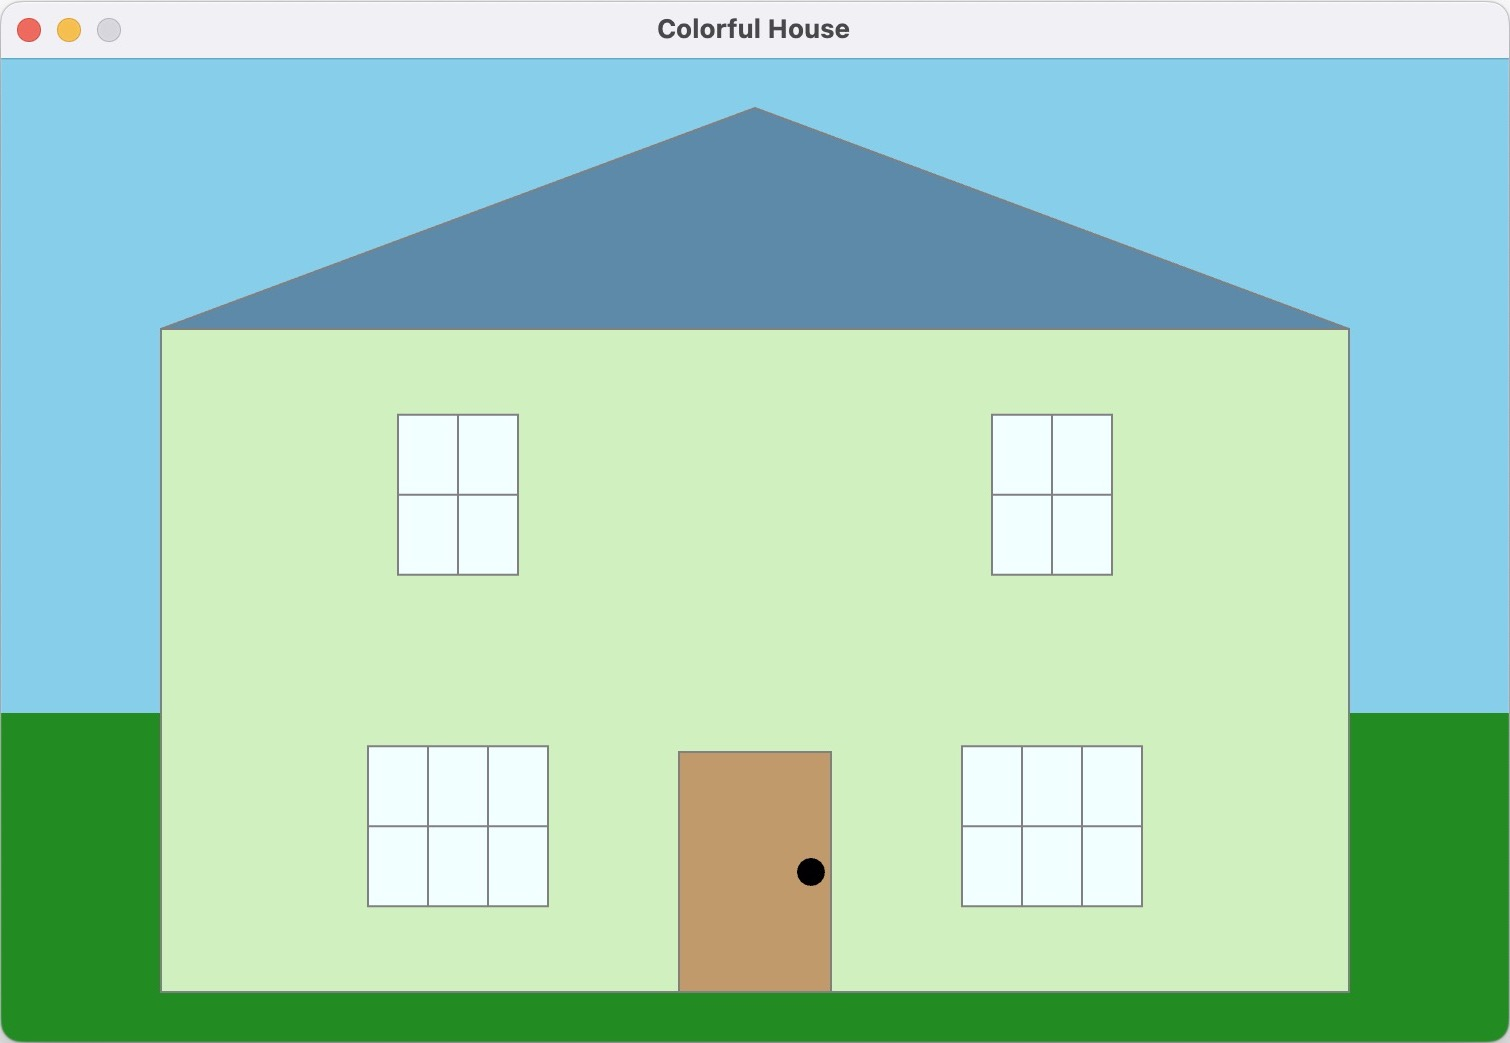
\includegraphics[width=.8\linewidth, trim={2mm 2mm 2mm 2mm},clip]{images/ch08/ColorfulHouse.jpg}};
    \drawshadow{image}
    
    % house (x, y)
    \draw[ultra thin,gray] (1.1,0.32)--(1.1,6.84);
    \draw[ultra thin,gray] (0,6.51)--(9.4,6.51);
    \draw[ultra thin,gray] (9.4,6.51)--(9.4,0.32);
    % dividers for wall
    \draw[ultra thin,gray] (1.1,2.62)--(9.4,2.62);
    \draw[ultra thin,gray] (5.24,0.32)--(5.24,4.94);
    \filldraw (1.1,6.51) circle (1pt) node [below right] {$(x,y)$};
    \filldraw (3.17,3.79) circle (1pt) node [below right] {$(x_1,y_1)$};
    \filldraw (2.75,4.34) circle (1pt) node [above] {$(left,top)$};
\end{tikzpicture}
\caption{ရောင်စုံအိမ်လေး} 
\label{fig:colorful_house}
\end{figure}

\subsection*{\fSubSecCodeBf{draw\_window}}
ပြတင်းပေါက်တွေဆွဲဖို့ \fCode{draw\_window} ဖန်ရှင် သတ်မှတ်သင့်တယ်။ ပြတင်းပေါက် အရွယ်အစား (မှန်ချပ်အရေအတွက်) ကို $rows \times columns$ နဲ့ ဖော်ပြနိုင်တယ်။  အပေါ်ပြတင်းပေါက် နှစ်ခုက $2 \times 2$ ဖြစ်ပြီး အောက်နှစ်ခုက $2 \times 3$ ။  အောက်ဖော်ပြပါ \fCode{draw\_window} မှာ \fCode{x}\fEn{,} \fCode{y}\fEn{,} \fCode{row}\fEn{,} \fCode{col} တို့ဟာ ပြတင်းပေါက် ဗဟိုမှတ်, အရွယ်အစားနဲ့ အရောင် တို့အတွက် ပါရာမီတာတွေဖြစ်တယ်။ နံရံ ပထမတစ်ပိုင်းရဲ့ ဗဟိုမှတ်ဟာ $(x_1, y_1)$ ဆိုပါစို့ (ပုံတွင်ကြည့်ပါ)။ ပြတင်းပေါက်ကို အခုလို

%
\begin{py}
draw_window(ß$x_1$ß, ß$y_1$ß, 2, 2);
\end{py}
%
ဆွဲနိုင်ပါတယ်။ နံရံတစ်ပိုင်းစီအတွက် ဗဟိုမှတ်ရှာတာ သိပ်မခက်ဘူး။ ဒါကြောင့် ဗဟိုမှတ်ကို ပါရာမီတာအနေနဲ့ ထားတာ အဆင်ပြေတယ်။ (ပြတင်းတစ်ပေါက်ချင်းအတွက်  သူ့ရဲ့ ဘယ်ဘက်အပေါ် ထောင့်\allowbreak စွန်းမှတ် $(x,y)$ တန်ဖိုးကို တွက်ကြည့်ပါ။ ဗဟိုမှတ်တွက်တာလောက် မလွယ်ကူတာ တွေ့ရလိမ့်မယ်)။ 

%
\begin{py}
# File: colorful_house.py
import arcade
from arcade.color import *

# x, y ß\fMM{က ပြတင်းပေါက် အလယ်မှတ်ပါ၊ ပုံထဲမှာ $(x_1, y_1)$ နဲ့ပြထားတယ်}  ß
def draw_window(x, y, row, col):
    pane_width = 30
    pane_height = 40
    window_width = pane_width * col
    window_height = pane_height * row
    top = y - window_height / 2
    left = x - window_width / 2
    for i in range(row):
        for j in range(col):
            arcade.draw_lrtb_rectangle_filled(left + pane_width * j,
                                              left + pane_width * (j+1),
                                              top + pane_height * (i+1),
                                              top + pane_height * i,
                                              AZURE_MIST)
            arcade.draw_lrtb_rectangle_outline(left + pane_width * j,
                                               left + pane_width * (j+1),
                                               top + pane_height * (i+1),
                                               top + pane_height * i,
                                               GRAY)
\end{py}
%
ပြတင်းပေါက် မှန်ချပ်တွေ ဆွဲတာက အခန်း (\fRefNo{\ref{ch:ch07ctlstmt}}) စာမျက်နှာ (\fRefNo{\pageref{lst:checkerboard}}) \fEn{checkerboard} လိုပါပဲ။ တကွက်ချင်းရဲ့ \fEn{left, right, top, bottom} တွေ \fEn{loop} တစ်ကျော့တိုင်းမှာ မှန်အောင်တွက်နိုင်ရင် ပြတင်းပေါက်ဆွဲလို့ ရမှာပါ။ မှန်တစ်ချပ် အကျယ်၊ အမြင့် $30, 40$ သတ်မှတ်တယ်။ ပြတင်းပေါက်တစ်ခုလုံး အကျယ်၊ အမြင့်ကို
\begin{codetxt}
window_width = pane_width * col
window_height = pane_height * row
\end{codetxt}
ဖော်မြူလာနဲ့ တွက်ရပါမယ်။ ပြတင်းပေါက် အလယ်မှတ် \fCode{x, y} ကနေ ဘယ်ဘက် အပေါ်ထောင့်စွန်းမှတ်ကို ရှာမယ်ဆိုရင်
\begin{codetxt}
top = y - window_height / 2
left = x - window_width / 2
\end{codetxt}
(ပုံကိုကြည့်ပြီး $x_1, y_1$ အမှတ်ကနေ $left, top$ အမှတ်ကို ဘယ်လိုရှာမလဲ စဉ်းစားကြည့်ပါ)။ မှန်ချပ်တစ်ချပ်ချင်း ကိုဩဒိနိတ်တွေကို \fCode{i} နဲ့  \fCode{j} (မှန်ချပ်ရဲ့ \fEn{row} နဲ့ \fEn{column} နံပါတ်) ပေါ်မူတည်ပြီး အခုလို တွက်လို့ရမယ်

\begin{py}
left + pane_width * j,          # ß\fMM{မှန်ချပ်ရဲ့} \fEn{left $x$}ß
left + pane_width * (j+1),      # ß\fMM{မှန်ချပ်ရဲ့} \fEn{right $x$}ß
top + pane_height * (i+1),      # ß\fMM{မှန်ချပ်ရဲ့} \fEn{bottom $y$}ß
top + pane_height * i,          # ß\fMM{မှန်ချပ်ရဲ့} \fEn{top $y$}ß
\end{py}
ဥပမာ $(left, top) = (100, 120)$ ဆိုပါစို့။ ညာဘက်အောက် မှန်ချပ်အတွက် \fCode{i = 1}\fEn{,} \fCode{j = 1} ဖြစ်တယ် (\fCode{i} နဲ့  \fCode{j} တန်ဖိုး သုညက စတယ်ဆိုတာ အမှတ်ရပါ)။ အဲဒီမှန်ချပ်ရဲ့ ကိုဩဒိနိတ်တွေက
\begin{codetxt}
100 + 30 * 1            = 130
100 + 30 * (1 + 1)      = 160 
120 + 40 * (1 + 1)      = 200
120 + 40 * 1            = 160
\end{codetxt}
ဖြစ်ပါတယ်။ 



\subsection*{\fSubSecCodeBf{draw\_house}}
\fCode{draw\_house} ကို အောက်ပါအတိုင်း သတ်မှတ်ထားတယ်။ \fCode{left} နဲ့ \fCode{top} က အိမ်တည်နေရာ $(x, y)$ လက်ခံတဲ့ ပါရာမီတာတွေပါ။ \fCode{width} နဲ့ \fCode{height} က အိမ်တစ်ခုလုံးရဲ့ အကျယ်နဲ့ အမြင့်အတွက်။ 
%
\begin{py}
# left ß$= x$ß top ß$= y$ \fMM{(ပုံတွင်ကြည့်ပါ)}ß
def draw_house(left, top, width, height):
    middle = left + width / 2
    wall_top = top + height / 4
    right = left + width
    wall_bottom = top + height

    arcade.draw_lrtb_rectangle_filled(left, right,
                                      wall_bottom, wall_top,
                                      TEA_GREEN)
    arcade.draw_lrtb_rectangle_outline(left, right,
                                       wall_bottom, wall_top,
                                       GRAY)

    arcade.draw_triangle_filled(left, wall_top, 
                                right, wall_top, 
                                middle, top,
                                AIR_FORCE_BLUE)
    arcade.draw_triangle_outline(left, wall_top,
                                 right, wall_top,
                                 middle, top,
                                 GRAY)

    left_windows_x = left + width/4
    right_windows_x = left + width * 3/4

    wall_height = height * 3/4
    upper_windows_y = wall_top + wall_height/4
    lower_windows_y = wall_top + wall_height/4 * 3

    draw_window(left_windows_x, upper_windows_y, 2, 2)
    draw_window(left_windows_x, lower_windows_y, 2, 3)
    draw_window(right_windows_x, upper_windows_y, 2, 2)
    draw_window(right_windows_x, lower_windows_y, 2, 3)

    door_width = 76
    door_height = 120
    door_top = wall_bottom - door_height
    door_left = left + width/2 - door_width/2
    draw_main_door(door_left, door_top, 
                   door_width, door_height, 
                   WOOD_BROWN)
\end{py}
%
အိမ်ခေါင်မိုး ထိပ်စွန်းမှတ်က အိမ်ကို အလယ်ကနေ ပိုင်းဖြတ်တဲ့ ဒေါင်လိုက်မျဉ်းပေါ်မှာပါ (ခေါက်ချိုးညီမျဉ်း)။ ဒီမျဉ်းပေါ်က $x$ အမှတ်ကို \fCode{middle} လို့ ထားမယ်။  သူ့တန်ဖိုးက
\begin{codetxt}
middle = left + width / 2
\end{codetxt}
ဖြစ်တယ်။ နံရံ အပေါ်အနားရဲ့ $y$ အမှတ်ကို \fCode{wall\_top} လို့ ထားတယ်။ သူ့တန်ဖိုးက
\begin{codetxt}
wall_top = top + height / 4
\end{codetxt}
ဖြစ်မယ်။ \fCode{top} ကို အိမ်အမြင့်ရဲ့ လေးပုံတစ်ပုံ ပေါင်းပေးရမှာပါ။ နံရံ အောက်ဘက်အနားရဲ့ $y$ အမှတ်ကို \fCode{wall\_bottom} လို့ ထားတယ်။ သူ့တန်ဖိုးက
\begin{codetxt}
wall_bottom = top + height
\end{codetxt}
နံရံ ညာဘက်အနားရဲ့ $x$ အမှတ်ကို \fCode{right} လို့ ထားတယ်။ သူ့တန်ဖိုးက
\begin{codetxt}
right = left + width
\end{codetxt}
(ရေပြင်ညီမျဉ်းပေါ်က အမှတ်အားလုံး $y$ တန်ဖိုး တူညီတယ်၊ ဒေါင်လိုက်မျဉ်းပေါ်က အမှတ်အားလုံး $x$ တန်ဖိုး တူညီတယ်လို့ သိထားပါ)။

ခေါင်မိုးကို \fCode{draw\_triangle\_filled} နဲ့ အခုလိုဆွဲနိုင်ပါတယ်။ တြိဂံရဲ့ ထောင့်စွန်းမှတ်တွေ ထည့်ပေးရမှာပါ။ (တြီဂံအနားသတ်ကို \fCode{draw\_triangle\_outline} နဲ့ ဆွဲတယ်။ ရှေ့စာမျက်နှာ \fCode{draw\_house} မှာ ကြည့်ပါ)။ 
\begin{py}
# draw roof 
arcade.draw_triangle_filled(left, wall_top,   # ß\fMM{ဘယ်ထောင့်စွန်း}ß
                            right, wall_top,  # ß\fMM{ညာထောင့်စွန်း}ß 
                            middle, top,      # ß\fMM{အပေါ်ထိပ်စွန်း}ß
                            AIR_FORCE_BLUE)
\end{py}



ပြတင်းပေါက်တွေရဲ့ အလယ်မှတ်တွေကို အောက်ပါအတိုင်း တွက်ထားတယ်။ ဘယ်ဘက် ပြတင်းနှစ်ပေါက် အလယ်မှတ် $x$ တန်ဖိုး တူတယ်။ ညာဘက်နှစ်ခု အလယ်မှတ်လည်း $x$ တန်ဖိုး တူတယ်။ အပေါ် ပြတင်းနှစ်ပေါက် အလယ်မှတ် $y$ တန်ဖိုး တူတယ်။ အောက်နှစ်ခု အလယ်မှတ်လည်း $y$ တန်ဖိုး တူတယ်။ နံရံအမြင့်က အိမ်အမြင့်ရဲ့ လေးပုံသုံးပုံ (ခေါင်မိုးက လေးပုံတစ်ပုံ ဖြစ်တဲ့အတွက်)။
%
\begin{py}
# center points of the windows
left_windows_x = left + width/4
right_windows_x = left + width * 3/4

wall_height = height * 3/4
upper_windows_y = wall_top + wall_height/4
lower_windows_y = wall_top + wall_height/4 * 3
\end{py}
%
ဒီအမှတ်တွေသိရင် ပြတင်းပေါက်တွေကို ဒီလိုဆွဲရုံပဲ 
%
\begin{py}
draw_window(left_windows_x, upper_windows_y, 2, 2)
draw_window(left_windows_x, lower_windows_y, 2, 3)
draw_window(right_windows_x, upper_windows_y, 2, 2)
draw_window(right_windows_x, lower_windows_y, 2, 3)
\end{py}
%
အိမ်တံခါးမ ကို အခုလို ဆွဲပါတယ်။ အမြင့်နဲ့ အကျယ်ကို ကြည့်ကောင်းအောင် သင့်တော်သလိုထားနိုင်တယ်။ နေရာအတွက် \fCode{door\_top}\fEn{,} \fCode{door\_left} တွက်တာလည်း မခက်ပါဘူး။ နားလည်မှာပါ။

%
\begin{py}
# draw main door
door_width = 76
door_height = 120
door_top = wall_bottom - door_height
door_left = left + width/2 - door_width/2
draw_main_door(door_left, door_top,
               door_width, door_height,
               WOOD_BROWN)
\end{py}
%
အတွက်အချက်တွေ အားလုံး ဒီလောက်ပါပဲ။ အရမ်းမခက်ဘူး ထင်ပါတယ်။ \fCode{draw\_house} ဖန်ရှင်တစ်ခုလုံး ရှေ့စာမျက်နှာမှာ အစအဆုံး ပြန်လေ့လာကြည့်ပါ။

\subsection*{\fSubSecCodeBf{draw\_main\_door}}
\fCode{draw\_main\_door} ဖန်ရှင်က ဒီလို $\ldots$ \fCode{left} နဲ့ \fCode{top} က တံခါးမ အပေါ်ဘယ်ဘက်ထောင့် အမှတ်ပါ။ တံခါးသော့ကို \fCode{draw\_circle\_filled} နဲ့  ဆွဲတယ်။ စက်ဝိုင်း ဗဟိုမှတ်ကို ထည့်ပေးရတယ်။ ဘယ်၊ ညာ၊ အထက်၊ အောက် ဘယ်လိုတွက်ထားလဲ အခုလောက်ဆို နားလည်လောက်ပြီလို့ ယူဆတယ်။ 
%
\begin{py}
def draw_main_door(left, top, width, height, color):
    arcade.draw_lrtb_rectangle_filled(left, left + width,
                                      top + height, top,
                                      color)
    arcade.draw_lrtb_rectangle_outline(left, left + width,
                                       top + height, top,
                                       GRAY)
    # draw door lock
    arcade.draw_circle_filled(left + width - 10,  # circle center x 
                              top + height/2,     # circle center y
                              7,                  # radius
                              BLACK)
\end{py}
%

အိမ်ပုံဆွဲတဲ့အခါ ခေါက်ချိုးညီ ပေါ်အောင်နဲ့ သင့်တော်တဲ့ အရွယ်အစားဖြစ်အောင် အခုလိုတွက်ထားပါတယ်
%
\begin{py}
WIN_WIDTH = 754
WIN_HEIGHT = 492
SIDE_MARGIN = 80
TOP_BTM_MARGIN = 25
HOUSE_WIDTH = WIN_WIDTH - 2 * SIDE_MARGIN
HOUSE_HEIGHT = WIN_HEIGHT - 2 * TOP_BTM_MARGIN
\end{py}
% 
ဝင်းဒိုး အကျယ်နဲ့ အမြင့် $754, 492$ \fEn{pixels} ထားတယ်။ ဝင်းဒိုးရဲ့ ဘယ်၊ ညာနဲ့ အထက်၊ အောက် ဘောင်တွေကနေ အိမ်ကို  $80, 25$ \fEn{pixels} ခွာထားတယ်။

နောက်ဆုံးတော့ \fEn{Arcade} လိုက်ဘရီ လိုအပ်ချက်အတိုင်း အခုလို တစ်ဆင့်ချင်း ပြင်ဆင်ပြီး  ရောင်စုံအိမ်ပုံလေး ဆွဲလို့ရပါပြီ
%
\begin{py}
arcade.open_window(WIN_WIDTH, WIN_HEIGHT, "Colorful House")
arcade.set_viewport(0, WIN_WIDTH, WIN_HEIGHT, 0)

# Set the background color
arcade.set_background_color(arcade.color.SKY_BLUE)

# Get ready to draw
arcade.start_render()

# ß\fMM{ဝင်းဒိုးအောက်ပိုင်း သုံးပုံတစ်ပုံ အစိမ်းရောင်ဖြစ်အောင် (မြက်ခင်းလေးပေါ့)}ß 
arcade.draw_lrtb_rectangle_filled(0, WIN_WIDTH, 
                                  WIN_HEIGHT, WIN_HEIGHT * 2/3, 
                                  FOREST_GREEN)
draw_house(SIDE_MARGIN, TOP_BTM_MARGIN, HOUSE_WIDTH, HOUSE_HEIGHT)

# Finish drawing
arcade.finish_render()

# Keep the window up until someone closes it.
arcade.run()
\end{py}
%
မှတ်ချက်။\qquad ။ အခန်း (\fRefNo{\ref{ch:ch07ctlstmt}}) စာမျက်နှာ (\fRefNo{\pageref{sec:python_arcade}}) မှာ \fEn{Arcade} လိုက်ဘရီအကြောင်း မိက်ဆက်ပေးထားပါတယ်။ အဲဒီအပိုင်းဖတ်ထားမှ အခုရှင်းပြတာတွေကို သေချာနားလည်နိုင်မှာပါ။ 

ရောင်စုံအိမ်လေးဆွဲတဲ့ ပရိုဂရမ်ကို တစ်ဆက်တည်း ဆက်စပ် ကြည့်လို့အဆင်ပြေအောင် အစအဆုံး ထည့်ပေးထားတယ်။ လေ့လာကြည့်ပါ။ 
%
\begin{py}
import arcade
from arcade.color import *


def draw_window(x, y, row, col):
    pane_width = 30
    pane_height = 40
    window_width = pane_width * col
    window_height = pane_height * row
    top = y - window_height / 2
    left = x - window_width / 2
    for i in range(row):
        for j in range(col):
            arcade.draw_lrtb_rectangle_filled(left + pane_width * j,
                                              left + pane_width * (j+1),
                                              top + pane_height * (i+1),
                                              top + pane_height * i,
                                              AZURE_MIST)
            arcade.draw_lrtb_rectangle_outline(left + pane_width * j,
                                               left + pane_width * (j+1),
                                               top + pane_height * (i+1),
                                               top + pane_height * i,
                                               GRAY)


def draw_main_door(left, top, width, height, color):
    arcade.draw_lrtb_rectangle_filled(left, left + width,
                                      top + height, top,
                                      color)
    arcade.draw_lrtb_rectangle_outline(left, left + width,
                                       top + height, top,
                                       GRAY)
    # draw door lock
    arcade.draw_circle_filled(left + width - 10,
                              top + height/2,
                              7,                  # radius
                              BLACK)


def draw_house(left, top, width, height):
    middle = left + width / 2
    wall_top = top + height / 4
    right = left + width
    wall_bottom = top + height

    arcade.draw_lrtb_rectangle_filled(left, right,
                                      wall_bottom, wall_top,
                                      TEA_GREEN)
    arcade.draw_lrtb_rectangle_outline(left, right,
                                       wall_bottom, wall_top,
                                       GRAY)

    arcade.draw_triangle_filled(left, wall_top, right,
                                wall_top, middle, top,
                                AIR_FORCE_BLUE)
    arcade.draw_triangle_outline(left, wall_top,
                                 right, wall_top,
                                 middle, top,
                                 GRAY)

    # center points of the windows
    left_windows_x = left + width/4
    right_windows_x = left + width * 3/4

    wall_height = height * 3/4
    upper_windows_y = wall_top + wall_height/4
    lower_windows_y = wall_top + wall_height/4 * 3

    draw_window(left_windows_x, upper_windows_y, 2, 2)
    draw_window(left_windows_x, lower_windows_y, 2, 3)
    draw_window(right_windows_x, upper_windows_y, 2, 2)
    draw_window(right_windows_x, lower_windows_y, 2, 3)

    # draw main door
    door_width = 76
    door_height = 120
    door_top = wall_bottom - door_height
    door_left = left + width/2 - door_width/2
    draw_main_door(door_left, door_top,
                   door_width, door_height,
                   WOOD_BROWN)

WIN_WIDTH = 754
WIN_HEIGHT = 492
SIDE_MARGIN = 80
TOP_BTM_MARGIN = 25
HOUSE_WIDTH = WIN_WIDTH - 2 * SIDE_MARGIN
HOUSE_HEIGHT = WIN_HEIGHT - 2 * TOP_BTM_MARGIN

# Open up a window.
# From the "arcade" library, use a function called "open_window"
# Set the window title to "Colorful House"
# Set the dimensions (width and height)
arcade.open_window(WIN_WIDTH, WIN_HEIGHT, "Colorful House")
arcade.set_viewport(0, WIN_WIDTH, WIN_HEIGHT, 0)

# Set the background color
arcade.set_background_color(arcade.color.SKY_BLUE)

# Get ready to draw
arcade.start_render()

arcade.draw_lrtb_rectangle_filled(0, WIN_WIDTH,
                                  WIN_HEIGHT, WIN_HEIGHT * 2 / 3,
                                  FOREST_GREEN)
draw_house(SIDE_MARGIN, TOP_BTM_MARGIN, HOUSE_WIDTH, HOUSE_HEIGHT)


# Finish drawing
arcade.finish_render()

# Keep the window up until someone closes it.
arcade.run()

\end{py}
%

\subsection*{ပိုကောင်းအောင် ပြုပြင်သင့်တဲ့ နေရာလေးတွေ}
ရောင်စုံအိမ်လေး ပရိုဂရမ်က အတန်အသင့် အဆင်ပြေနေပါပြီ။ တချို့နေရာလေးတွေ ပိုကောင်းအောင် \fEn{improve} လုပ်လို့ရပါတယ်။ ပြင်ဖို့က သိပ်လည်းမခက်ဘူး။ ထောင့်မှန်စတုဂံတွေကို နှစ်ခါဆွဲနေရတယ်။ အရောင်ဖြည့်ဖို့ \fCode{draw\_lrtb\_rectangle\_filled} နဲ့တစ်ခါ အနားသတ်အတွက် \fCode{draw\_lrtb\_rect\allowbreak angle\_outline} နဲ့တစ်ခါ။ ဖန်ရှင်မှာ ထည့်ပေးတဲ့ တန်ဖိုးတွေကလည်း အားလုံး တူတူပဲ (အရောင်ကလွဲလို့)။ အခုလို ဖန်ရှင် သတ်မှတ်ထားလိုက်ရင် ပိုအဆင်ပြေသွားမှာပါ
%
\begin{py}
def draw_rect_filled_with_outline(left, right, top, bottom, color):
    arcade.draw_lrtb_rectangle_filled(left, right, top, bottom, color)
    arcade.draw_lrtb_rectangle_outline(left, right, top, bottom, GRAY)
\end{py}
%
မီးခိုးရောင် အနားသတ်နဲ့ \fEn{rectangle} ကို အရောင်အမျိုးမျိုး ဖြည့်ဆွဲလို့ရမှာပါ။ ဥပမာ \fCode{draw\_window} မှာ အခုလို သုံးလို့ရမယ်
%
\begin{py}
draw_rect_filled_with_outline(left + pane_width * j,
                              left + pane_width * (j+1),
                              top + pane_height * (i+1),
                              top + pane_height * i,
                              AZURE_MIST)
\end{py}
%
နံရံနဲ့ တံခါးမဆွဲရင်လည်း အလားတူ သုံးရုံပဲ။

\section{ပါရာမီတာ ရွေးချယ်သတ်မှတ်ခြင်း}
ဖန်ရှင်သတ်မှတ်တဲ့အခါ ‘ဘယ်ဟာတွေက ပါရာမီတာ ဖြစ်သင့်လဲ’၊ ‘ဘယ်ဟာတွေကတော့ရော  မဖြစ်သင့်ဘူးလား’ ဝေခွဲဆုံးဖြတ်မရ ဖြစ်လေ့ရှိတာဟာ စလေ့လာတဲ့သူတွေရော အတွေ့အကြုံရှိပြီး သူတွေအတွက်ပါ ပုံမှန် ဖြစ်ရိုးဖြစ်စဉ် တစ်ခုပါပဲ။ ဖော်မြူလာ ရှိပြီးသား သင်္ချာဖန်ရှင်တွေအတွက်တော့ သိပ်ခေါင်းစားစရာ မလိုပါဘူး။ စက်ဝိုင်းဧရိယာရှာရင် အချင်းဝက်၊ တြိဂံဆိုရင် အခြေနဲ့ အမြင့်တို့ကို ပါရာမီတာ အနေနဲ့ ထားရမယ်ဆိုတာ သိသာတယ်။ ဒါပေမဲ့ တချို့နေရာတွေမှာ ထင်သလောက် မရိုးရှင်းပါဘူး။ 

ယေဘုယျအားဖြင့် ဖန်ရှင် ခေါ်တဲ့အခါကျတော့မှ တန်ဖိုးထည့်ပေးချင်တဲ့ အရာတွေကို ပါရာမီတာ အနေနဲ့ ထားလေ့ရှိတယ်။ ရောင်စုံအိမ်လေးမှာ \fCode{draw\_window} ဖန်ရှင်ခေါ်တော့မှ ဆွဲမဲ့ ပြတင်းပေါက် တည်နေရာနဲ့ \fEn{row} နဲ့ \fEn{column} အရေအတွက် ထည့်ပေးရမှာပါ။ ဒီတော့မှ လိုချင်တဲ့နေရာမှာ လိုချင်တဲ့ \fEn{row, column} အရေအတွက်နဲ့ ဆွဲလို့ရမယ်။

အခုလက်ရှိ \fCode{draw\_window} ဟာ ပြတင်းပေါက်အရောင် တစ်မျိုးနဲ့ပဲ ဆွဲလိုရနိုင်မယ်။ အကယ်၍ အပေါ်ပြတင်းပေါက် နှစ်ခုနဲ့ အောက်ပြတင်းပေါက် နှစ်ခု အရောင်ကွဲနေတယ်ဆိုပါစို့။ ဒါဆိုရင်တော့ \fCode{draw\allowbreak\_window} ကို အခုလို ပြင်ပေးရပါမယ်

%
\begin{py}
def draw_window(x, y, row, col, ß\textbf{color}ß):
    # ß$\ldots$ \fMM{ဒီနေရာက လိုင်းတွေ တချို့ကို ချန်ထားတယ်}ß
    for i in range(row):
        for j in range(col):
            draw_rect_filled_with_outline(left + pane_width * j,
                                          left + pane_width * (j+1),
                                          top + pane_height * (i+1),
                                          top + pane_height * i,
                                          ß\textbf{color}ß)
\end{py}
%
အပေါ်ကို အဖြူရောင်၊ အောက်ကို မီးခိုး ဆွဲမယ်ဆိုရင်
%
\begin{py}
draw_window(left_windows_x, upper_windows_y, 2, 2, WHITE)
draw_window(right_windows_x, upper_windows_y, 2, 2, WHITE)
draw_window(left_windows_x, lower_windows_y, 2, 3, GRAY)
draw_window(right_windows_x, lower_windows_y, 2, 3, GRAY)
\end{py}
%
ဒီလိုဆွဲလို့ ရပါတယ်။

တကယ်လို့ မှန်ချပ်အရွယ်ပါ ဖန်ရှင်ခေါ်တဲ့အခါကျတော့မှ သတ်မှတ်လို့ရချင်ရင် မှန်ချပ် အကျယ်၊ အမြင့် အတွက် ပါရာမီတာနှစ်ခု ထပ်ထည့်နိုင်ပါတယ်
%
\begin{py}
def draw_window(x, y, row, col, color, ß\textbf{pane\_width}ß, ß\textbf{pane\_height}ß):
    # pane_width = 30  ß\fMM{ဒီနှစ်ကြောင်း မလိုတော့ဘူး}ß
    # pane_height = 40
    window_width = pane_width * col
    window_height = pane_height * row
    top = y - window_height / 2
    left = x - window_width / 2
    for i in range(row):
        for j in range(col):
            draw_rect_filled_with_outline(left + pane_width * j,
                                          left + pane_width * (j+1),
                                          top + pane_height * (i+1),
                                          top + pane_height * i,
                                          color)
\end{py}
%
ပါရာမီတာတွေ ထပ်ဖြည့်ခြင်းအားဖြင့် ပြတင်းပေါက်ကို အရောင် အမျိုးမျိုးနဲ့ ဆွဲလို့ရလာတယ်။ မှန်ချပ်အရွယ် အမျိုးမျိုးနဲ့ ဆွဲလို့ရလာတယ်။ ဖန်ရှင်ဟာ ပိုပြီး ဂျန်နရယ်ကျလာတယ်၊ \fEn{flexible} ပိုဖြစ်လာတယ်။ ဒီတော့ တတ်နိုင်သမျှ ပါရာမီတာတွေ များများထားရင် ပိုကောင်းတယ် ယူဆရမှာလား။ ပါရာမီတာတွေ များလာတာနဲ့အမျှ သူတို့ကို ဘာအတွက်ထည့်ရတာလဲ၊ ဘာတန်ဖိုးထည့်သင့်လဲ စဉ်းစားဖို့လိုလာတယ်။ ဖန်ရှင်ကို အသုံးပြုရတာ ပိုခက်လာတယ်။ ဒါကြောင့် \fEn{flexibility} နဲ့ အသုံးပြုရ လွယ်ကူမှု ပေါ်မူတည်ပြီး ချင့်ချိန်သတ်မှတ်ရမှာပါ။

ဂျန်နရယ်ကျတဲ့၊ \fEn{flexible} ဖြစ်တဲ့ ဖန်ရှင်တစ်ခုကို အခြေခံပြီး \fEn{specific} ဖြစ်တဲ့ ဖန်ရှင်တွေကို သတ်မှတ်ယူလို့ရတယ်။ ဒီဖန်ရှင်နှစ်ခုမှာ အပေါ်က \fCode{draw\_window} ကို ပြန်သုံးထားပါတယ်။
%
\begin{py}
def draw_2x2_pearl_window(x, y):
    draw_window(x, y, 2, 2, PEARL, 30, 40)

def draw_2x3_gray_window(x, y):
    draw_window(x, y, 2, 3, LIGHT_GRAY, 30, 40)
\end{py}
%
$2 \times 2$ ပုလဲရောင်နဲ့ $2 \times 3$ မီးခိုးရောင် ပြတင်းပေါက်ဆွဲဖို့ပါ။ နေရာအတွက် ပါရာမီတာ နှစ်ခုပဲ ပါတော့တယ်။ သုံးရတာ ပိုလွယ်သွားတာ သိသိသာသာတွေ့ရမှာပါ။ ဥပမာ ရောင်စုံအိမ်လေးမှာ အပေါ်ပြတင်းနှစ်ပေါက်ကို ပုလဲရောင်၊ အောက်နှစ်ခုကို မီးခိုးရောင် လိုချင်ရင် အခုလို ဆွဲရုံပါပဲ
%
\begin{py}
draw_2x2_pearl(left_windows_x, upper_windows_y)
draw_2x3_gray(left_windows_x, lower_windows_y)
draw_2x2_pearl(right_windows_x, upper_windows_y)
draw_2x3_gray(right_windows_x, lower_windows_y)
\end{py}
%
အရောင်နဲ့ \fEn{row, column} တော့ ပြောင်းချင်လို့ မရဘူး။ ပုံသေ ဒီနှစ်မျိုးပဲ ရပါမယ်။ ဒါကြောင့် \fEn{flexibility} အရတော့ အားနည်းတယ်ပေါ့။ ဒါပေမဲ့ သုံးရတာ အတော်လေးလွယ်တယ်။ ဂျန်နရယ်ကျတဲ့၊ \fEn{flexible} ဖြစ်တဲ့ ဖန်ရှင်ကို အခြေခံပြီး \fEn{specific} ဖြစ်တဲ့ ဖန်ရှင် သတ်မှတ်တဲ့ နည်းလမ်းကို ပရိုဂရမ်မာတွေ မကြာခဏ အသုံးပြုလေ့ရှိတယ်။ ကိုယ်တိုင် အသုံးချတတ်အောင် လေ့လာထားသင့်ပါတယ်။ အသုံးတည့်မှာပါ။ နားလည်ဖို့ သိပ်ခက်ခဲတဲ့ ကိစ္စလည်း မဟုတ်ပါဘူး။


\section{တန်ဖိုး ပြန်ပေးခြင်း၊ မပေးခြင်း}
တချို့ ဖန်ရှင်တွေမှာ တန်ဖိုးပြန်ပေးသင့် (သို့) မပေးသင့် ဆုံးဖြတ်ရ ခက်တတ်ပါတယ်။ ဒါနဲ့ပါတ်သက်ပြီး  ပထမဆုံး သိထားသင့်တာကတော့ တန်ဖိုး ပြန်ပေးခြင်း (သို့) မပေးခြင်းရဲ့ အကျိုးဆက်က ဘယ်လိုရှိမလဲ ဆိုတာပါ။
%
\begin{py}
def greet_guest_nort(guest_name):
    print(f'Hello, {guest_name}.')

def greet_guest_rt(guest_name):
    return f'Hello, {guest_name}.'
\end{py}
%
ဒီဖန်ရှင်နှစ်ခုက သဘောတရား ဆင်တူပါတယ်။ ကွာခြားတာဆိုလို့ ပထမတစ်ခုက တစ်ခါတည်း \fCode{print} နဲ့ စာသားကို \fEn{output} ထုတ်ပေးပြီး နောက်တစ်ခုကတော့ စာသားကိုပဲ \fEn{return} ပြန်ပေးတယ်။ ဒုတိယတစ်ခုနဲ့ စခရင်မှာထုတ်ချက်ရင်
%
\begin{py}
print(greet_guest_rt("Joe"))
\end{py}
%
ဖန်ရှင်ခေါ်တဲ့သူက \fCode{print} လုပ်ပေးရပါမယ်။ သုံးတဲ့သူအနေနဲ့တော့ အလုပ်ပိုတာပေါ့။ ဒါပေမဲ့ ဖန်ရှင်က ပြန်ရတဲ့ တန်ဖိုးကို လိုအပ်သလို ဆက်လက် အသုံးပြုနိုင်တယ်။ ဥပမာ \fEn{greet} လုပ်ပြီးရင် နေကောင်းလား ဆက်မေးချင်တယ်၊ ဒါမှမဟုတ် စာသားထဲက အက္ခရာ/စကားလုံး အစားထိုးမယ် ဆိုပါစို့
%
\begin{py}
print(greet_guest_rt("Joe") + '\nHow are you doing?')
print(greet_guest_rt('Kathy').replace('.', '!!!'))
\end{py}
%
ဖန်ရှင်ခေါ်တဲ့သူက ပြန်ရတဲ့ တန်ဖိုးကို လိုအပ်သလို ဆက်လက် အသုံးပြုလို့ ရပါမယ်။ တန်ဖိုးပြန်မရရင်တော့ ဒီလိုလုပ်လို့ ရမှာ မဟုတ်ပါဘူး။

နောက်တစ်ခုက တန်ဖိုးပြန်ပေးရင် မှန်/မမှန်စစ် \fEn{(test)} လုပ်ရတာ ပိုလွယ်တယ်။ ဒါက စာမျက်နှာ (\fRefNo{\pageref{lst:christmastree1}}) က ခရစ်စမတ် သစ်ပင်လေးကို ဖန်ရှင်ရေးထားတာပါ
%
\begin{py}
def christmas_tree(leaf_rows, trunk_rows):
    tree = []
    for r in range(leaf_rows):
        tree_row = ' ' * (leaf_rows - 1 - r)
        tree_row += '*' * (r * 2 + 1)
        tree.append(tree_row)
    trunk_width = 3
    for r in range(trunk_rows):
        tree_row = ' ' * (leaf_rows - 2)
        tree_row += '*' * trunk_width
        tree.append(tree_row)

    return tree
\end{py}
%
\fEn{Row} တစ်ခုချင်းကို \fEn{string} အနေနဲ့ \fEn{list} ထဲမှာ ထည့်ပြီး \fEn{return} ပြန်ပေးထားတယ်။ \fEn{Output} ထုတ်မယ်ဆိုရင်
%
\begin{py}
my_tree = christmas_tree(8, 4)
for row in my_tree:
    print(row)
\end{py}
%
ဒီဖန်ရှင် မှန်/မမှန် \fEn{test} လုပ်ဖို့ အခုလို ဖန်ရှင်တစ်ခု ရေးထားနိုင်ပါတယ်။  
%
\begin{py}
def test_christmas_tree():
    test_tree = [
        '    *',
        '   ***',
        '  *****',
        ' *******',
        '*********',
        '   ***',
        '   ***',
        '   ***',
    ]
    result_tree = christmas_tree(5, 3)
    if result_tree != test_tree:
        print("Error: expected and actual result don't match!")
    else:
        print("Expected and actual result do match!")
\end{py}
%
အကြောင်းတစ်ခုခုကြောင့် \fCode{christmas\_tree} ရဲ့ အတွင်းပိုင်း တည်ဆောက်ထားပုံကို (ပိုမြန်အောင်၊ ဒါမှမဟုတ် ပိုနားလည်ရ လွယ်ကူအောင်) ပြင်ရေးမယ်ဆိုရင် ရလဒ် နဂိုအတိုင်း ဖြစ်မဖြစ် ပြန်စစ်ဖို့ လိုပါတယ်။    တကယ်လို့ \fCode{christmas\_tree} က တန်ဖိုးပြန်မပေးဘဲ တစ်ခါတည်း  \fCode{print} ထုတ်လိုက်ရင် စခရင်မှာ ပေါ်လာတဲ့ \fEn{output} ကိုကြည့်ပြီး လူကိုယ်တိုင် စစ်ဆေးမှပဲ မှန်/မမှန်  သိနိုင်မှာပါ။ ပရိုဂရမ်ရေးပြီး အခုလို \fEn{automated testing} (လူက \fEn{test} မလုပ်ဘဲ ပရိုဂရမ်နဲ့ပဲ \fEn{test} လုပ်တာကို ဆိုလို) လုပ်ဖို့ မဖြစ်နိုင်ဘူး။ 

အခုဖော်ပြခဲ့သလို \fEn{testing} လုပ်တာဟာ \fEnEmp{unit testing} ရဲ့ အခြေခံသဘောတရားပါပဲ။ ဖန်ရှင်တစ်ခု (သို့) မော်ဒျူးတစ်ခုကို သူ့ချည်းသီးခြား မှန်/မမှန် \fEn{test} လုပ်တာကို \fEn{unit testing} လို့ ခေါ်တာပါ။ တန်ဖိုးပြန်ပေးတဲ့ ဖန်ရှင်တွေဟာ \fEn{unit test} လုပ်ရ လွယ်ကူတာ တွေ့နိုင်ပါတယ်။ ဆော့ဖ်ဝဲတည်ဆောက်ရာမှာ \fEnEmp{unit testing} ဟာ အရေးကြီးတဲ့ အခန်းကဏ္ဍတစ်ခု အနေနဲ့ ပါဝင်တယ်။ ကျယ်ပြန်တဲ့ နယ်ပယ်ဖြစ်ပြီး သီးခြားလေ့လာဖို့ လိုအပ်ပါတယ်။ ဒီစာအုပ်မှာတော့  ဖန်ရှင်တန်ဖိုး ပြန်ပေးခြင်းနဲ့ ဆက်စပ်နေတဲ့အတွက် အခြေခံလောက်လေးကိုပဲ ဗဟုသုတအနေနဲ့ ထည့်သွင်းဖော်ပြတာပါ။

\section{\fSecCodeBf{return}}
\fCode{return} ဟာ ဖန်ရှင်ကနေ သူ့ကိုခေါ်တဲ့သူ (သို့) ခေါ်ထားတဲ့နေရာဆီ ပြန်ရောက်သွားစေတယ်လို့ သိထားပြီးပြီ။ သတိပြုမိသင့်တဲ့ အသေးစိတ်အချက် တချို့ကို ဆက်ကြည့်ရအောင်။ \fCode{get\_sign} နဲ့ \fCode{print\_sign} ကို \fEn{cascading} \fCode{if} မသုံးဘဲ အခုလိုရေးလိုရပါတယ်
%
\begin{py}
def get_sign(r):
    if r > 0:
        return 'positive'
    if r < 0:
        return 'negative'

    return 'zero/nosign'

def print_sign(r):
    if r > 0:
        print('positive')
        return
    if r < 0:
        print('negative')
        return

    print('zero/nosign')
    return # ß\fMM{ဒါမပါလည်းရတယ်}ß
\end{py}
%
ရိုးရိုး \fCode{if} သုံးထားပေမဲ့ ကွန်ဒီရှင်မှန်ရင် \fCode{return} ဖြစ်သွားမှာမို့လို့ အောက်ကို မရောက်တော့ဘူး။ ဒီအတွက် \fEn{cascading} \fCode{if} အလုပ်လုပ်ပုံလိုပဲ ဖြစ်သွားတယ်။ အပေါ်မှာ မှန်ရင်အောက်ကို မရောက်လာနိုင်ဘူး။ အောက်က \fCode{if} တွေကို ရောက်လာတာဟာ အပေါ်က ကွန်ဒီရှင်တွေ မှားလို့ပဲ။ (အခုလိုမျိုးရေးသင့်တယ်လို့ မဆိုလိုပါ၊ \fCode{return} ရဲ့ သဘောတရားကို သတိပြုမိအောင် ဥပမာပြတာပါ)။


ဖန်ရှင်မှာ \fEn{loop} ထဲကနေ \fCode{return} လုပ်လိုက်ရင် \fEn{loop} ကို \fCode{break} လိုက်သလို ဖန်ရှင်ခေါ်တဲ့နေရာဆီကိုလည်း ပြန်ရောက်သွားမှာပါ။
%
\begin{py}
def read_int(prompt):
    while True:
        valin = input(prompt)
        try:
            return int(valin)
        except ValueError as err:
            if valin == 'quit':
                return
            print('Non-integer data!')


num = read_int('Enter number: ')
print(num)
\end{py}
%

\subsection*{မတော်တဆ \fSubSecCodeBf{None return} ဖြစ်ခြင်း}
အောက်ပါ ပကတိတန်ဖိုး ဖန်ရှင်မှာ \fCode{n} တန်ဖိုး သုညအတွက် မစစ်မိထားဘူး။ 
%
\begin{py}
def my_abs(n):
    if n > 0:
        return n
    elif n < 0:
        return -n
\end{py}
%
အကယ်၍ \fCode{print(my\_abs(0))} နဲ့ ထုတ်ကြည့်ရင် \fCode{None} လို့ ပြပါလိမ့်မယ်။ \fCode{n} သုညဖြစ်တဲ့အတွက် \fCode{if...elif} ထဲက \fCode{return} နှစ်ခုလုံး  မလုပ်ဘူး။ ဒီတော့ \fCode{if...elif} အပြီး နောက်တစ်ကြောင်းကို ရောက်လာတဲ့ သဘောပဲ။ ဖန်ရှင်ဘလောက်အဆုံးထိ ရောက်လာပြီးရင် ခေါ်ခဲ့တဲ့နေရာကို ပြန်သွားဖို့ \fCode{return} (နောက်မှာ တန်ဖိုးမပါ) လုပ်တယ်လို့ ယူဆရမှာပါ။ တန်ဖိုးမပါတဲ့ \fCode{return} က \fCode{None} ကို ပြန်ပေးပါတယ်။ ဒီလောက်ဆိုရင် ဘာလို့ \fCode{print(my\_abs(0))} က \fCode{None} ရတာလဲ နားလည်းမှာပါ။ ဒီအမှားကို ပြင်ထားတဲ့ ဥပမာနှစ်ခုကို ပြထားပါတယ်။ ဒုတိယတစ်ခုက အတွေ့အကြုံရှိတဲ့ \fEn{Python} ပရိုဂရမ်မာတစ်ယောက် ရေးလေ့ရှိတဲ့နည်း။ \fEn{Pythonic} ပိုဖြစ်တယ် (\fEn{Python} ပိုဆန်တယ်) ပေါ့။

%
\begin{py}
def my_abs(n):
    if n > 0:
        return n
    elif n < 0:
        return -n
    else:
        return 0
\end{py}
%
\betweenminted{\medskipamount}
%
\begin{py}
def my_abs(n):
    if n < 0:
        return -n
    return n
\end{py}
%


%။  ဒီနေရာမှာ စဉ်းစားစရာရှိလာတာက \fCode{calc\_age} က အထက်ဖော်ပြပါ ဖော့မတ်အမျိုးမျိုးကို လက်ခံပြီး အသက်ကို တွက်ပေးသင့်သလား၊ ဒါမှမဟုတ် ဖော့မတ်အမျိုးမျိုးကနေ \fCode{date} ပြောင်းဖို့အတွက် အခြားဖန်ရှင်တစ်ခု ထားသင့်သလား (ဥပမာ \fCode{parse\_date\_str})။ မက်သဒ်ဆိုင်ရာ ဂိုက်ဒ်လိုင်းတစ်ခုက ‘မက်သဒ်တစ်ခုဟာ အလုပ်တစ်ခုကိုပဲ မှန်ကန်အောင် ပီပီပြင်ပြင် ဆောင်ရွက်သင့်တယ်’ လို့ ဆိုပါတယ်။ မက်သဒ်တစ်ခုဟာ တာဝန်တွေ အများကြီးကို မဆောက်ရွက်သင့်ဘူး။ ဒီအချက်အရ \fCode{calcAge} နဲ့ \fCode{parseDateStr} နှစ်ခုသတ်မှတ်သင့်ပါတယ်။


